\chapter{Rare Languages}
\label{ch:rare-langs}



\setlength{\epigraphwidth}{5.6in} 
\epigraph{\textit{``Vasudhaiva Kutumbakam" (The entire world is a family) } --- Maha Upanishad }



%Neural machine translation (NMT)~\cite{bahdanau2014nmtattn,vaswani-2017-attention} 
NMT has progressed to reach human performance on select benchmark tasks~\cite{barrault-etal-2019-findings,barrault-etal-2020-findings}. 
However, as MT research has mainly focused on translation between a few high resource languages, the unavailability of usable-quality translation models for low resource languages remains an ongoing concern.
Even those commercial translation services attempting to broaden their language coverage has only reached around one hundred languages; this excludes most of the thousands of languages used around the world today.

Freely available corpora of parallel data for many languages are available, though they are hosted at various sites, and are in various forms. A challenge for incorporating more languages into MT models is a lack of easy access to all of these datasets. While standards like ISO 639-3 have been established to bring consistency to the labeling of language resources, these are not yet widely adopted.
In addition, scaling experimentation to several hundred languages on large corpora involves a significant engineering effort.
Simple tasks such as dataset preparation, vocabulary creation, transformation of sentences into sequences, and training data selection becomes formidable at scale due to corpus size and heterogeneity of data sources and file formats.
We have developed tools to precisely address all these challenges, which we demonstrate in this work.
 
Specifically, we offer three tools which can be used either independently or in combination to advance NMT research on a wider set of languages (Section \ref{sec:tools}): firstly, \mtdata, which helps to easily obtain parallel datasets (Section \ref{sec:mtdata}); secondly, \nlcodec, a vocabulary manager and storage layer for transforming sentences to integer sequences, that is efficient and scalable (Section \ref{sec:nlcodec}); and lastly, \rtg, a feature-rich PyTorch-backed NMT toolkit that supports reproducible experiments (Section \ref{sec:rtg}).

We demonstrate the capabilities of our tools by preparing a massive bitext dataset with more than 9 billion tokens per side, and training a single multilingual NMT model capable of translating 500 source languages to English (Section \ref{sec:500-eng}).
We show that the multilingual model is usable either as a service for translating several hundred languages to English (Section \ref{sec:value.off-shelf-mt}), or as a parent model in a transfer learning setting for improving translation of low resource languages~(Section~\ref{sec:value.transfer-learning}). 
%pretrained multilingual embeddings (Section \ref{sec:value.embeddings}),


\section{Tools}
\label{sec:tools}
 Our tools are organized into the following sections:

\begin{comment}
Specifically, \textsc{MTData} (Section \ref{sec:mtdata}) is useful for preparing training data for hundreds of languages, 
\textsc{NLCodec} (section \ref{sec:nlcodec}) is useful for efficiently preprocessing, storing, and accessing the training data,
and \textsc{RTG} (section \ref{sec:rtg}) NMT toolkit for training an MT model. 
In addition, all these tools are built with reproducibility and usability in mind. 
These tools have been made publicly available, with permissive open source licenses.
We hope these tools help advance MT efforts beyond the top few high resource languages. 
\end{comment}

\subsection{\textsc{MTData}}
\label{sec:mtdata}
\textsc{MTData} addresses an important yet often overlooked challenge -- dataset preparation. 
By assigning an ID for datasets, we establish a clear way of communicating the exact datasets used for MT experiments, which helps in reproducing the experimental setup.
By offering a unified interface to datasets from many heterogeneous sources, \mtdata\ hides mundane tasks such as locating URLs, downloading, decompression, parsing, and sanity checking. Some noteworthy features are:
\begin{itemize}[noitemsep,topsep=0pt,leftmargin=4mm]
\item \textit{Indexer}: a large index of publicly available parallel datasets.
\item \textit{ID Standardization:} creates standardized IDs for datasets, along with language IDs normalized to BCP-47 like codes; more details in section \ref{sec:did-bcp47}. 
\item \textit{Parsers:} parses heterogeneous data formats for parallel datasets, and produces a simple plain text file by merging all the selected datasets.
\item \textit{Extensible:} new datasets and parsers can be easily added.
\item \textit{Local Cache}: reduces network transfers by maintaining a local cache, which is shared between experiments.
\item \textit{Sanity Checker}: performs basic sanity checks such as segment count matching and empty segment removal. When error states are detected, stops the setup with useful error messages.
\item \textit{Reproducible:} stores a signature file that can be used to recreate the dataset at a later time.
\item \textit{Courtesy:} shows the original \BibTeX\ citation attributed to datasets.
\item \textit{Easy Setup:} \texttt{pip install mtdata}
\item \textit{Open-source:} \url{https://github.com/thammegowda/mtdata}
\end{itemize}

Listing \ref{lst:mtdata-eg} shows an example for listing and getting datasets for German-English.
\begin{listing}
\begin{minted}[baselinestretch=1, fontsize=\normalsize, frame=lines, framesep=2mm,]{bash}
# List all the available datasets for deu-eng
$ mtdata list -l deu-eng
# Get the selected training & held-out sets
$ mtdata get -l deu-eng  -o data -ts Statmt-newstest_deen-201{8,9}-deu-eng \ 
  -tr Statmt-commoncrawl_wmt13-1-deu-eng Statmt-europarl-10-deu-eng \ 
      Statmt-news_commentary-16-deu-eng --merge
\end{minted}
\caption{\mtdata\ commands for listing and downloading German-English datasets (Tested on v0.3.4).
The \texttt{--merge} flag results in merging all the training datasets specified by \texttt{-tr} argument into a single file. }
\label{lst:mtdata-eg}
\end{listing}
 In Section~\ref{sec:datasets}, we use \mtdata to obtain thousands of publicly available datasets for a large many-to-English translation experiment.

\subsection{\nlcodec}
\label{sec:nlcodec}
\nlcodec\ is a vocabulary manager with encoding-decoding schemes to transform natural language sentences to and from integer sequences.\\
\textbf{Features:}
\begin{itemize}[noitemsep,topsep=0pt,leftmargin=4mm]
\item \textit{Versatile:} Supports commonly used vocabulary schemes such as characters, words, and byte-pair-encoding (BPE) subwords~\cite{sennrich-etal-2016-bpe}.
\item \textit{Scalable:} Apache Spark\footnote{\url{https://spark.apache.org/}}\cite{zaharia2016spark} backend can be optionally used to create a vocabulary from massive datasets.
\item \textit{Easy Setup:} \texttt{pip install nlcodec} 
\item \textit{Open-source:}\\ \url{https://github.com/isi-nlp/nlcodec/}
\end{itemize}

When the training datasets are too big to be kept in the primary random access memory (RAM), the use of secondary storage is inevitable.
The training processes requiring random examples lead to random access from a secondary storage device.
Even though the latest advancements in secondary storage technology such as solid-state drive (SSD) have faster serial reads and writes, their random access speeds are significantly lower than that of RAM. 
%In addition, since sentences are of variable lengths, use of fixed sized tensors are not feasible. 
To address these problems, we include an efficient storage and retrieval layer, \nldb, which has the following features:
\begin{itemize}[noitemsep,topsep=0pt,leftmargin=4mm]
  \item \textit{Memory efficient} by adapting data types based on vocabulary size. For instance, encoding with vocabulary size less than 256 (such as characters) can be efficiently represented using 1-byte unsigned integers. Vocabularies with fewer than 65,536 types, such as might be generated when using subword models \cite{sennrich-etal-2016-bpe} require only 2-byte unsigned integers, and 4-byte unsigned integers are sufficient for vocabularies up to 4 billion types. 
As the default implementation of Python, CPython, uses 28 bytes for all integers, we accomplish this using NumPy~\cite{harris2020numpy}. This optimization makes it possible to hold a large chunk of training data in smaller RAM, enabling fast random access.
  \item \textit{Parallelizable:} Offers a multipart database by horizontal sharding that supports parallel writes (e.g., Apache Spark) and parallel reads (e.g., distributed training).
%  \item \textit{I/O efficient:} Reads and writes large blocks at once instead of multiple smaller chunks, thus taking advantage of faster serial reads and write speeds.
  \item Supports commonly used batching mechanisms, such as random batches with approximately-equal-length sequences.
\end{itemize}

\nldb\ has a minimal footprint and is part of the \nlcodec\ package.
In Section~\ref{sec:500-eng}, we take advantage of the scalability and efficiency aspects of \nlcodec\ and \nldb\ to process a large parallel dataset with 9 billion tokens on each side.


\subsection{\rtg}
\label{sec:rtg}
Reader translator generator (\rtg) is a neural machine translation (NMT) toolkit based on Pytorch~\cite{NEURIPS2019_Pytorch}. 
Notable features of \rtg\ are:
\begin{itemize}[noitemsep,topsep=0pt,leftmargin=4mm]
\item \textit{Reproducible:} All the required parameters of an experiment are included in a single YAML configuration file, which can be easily stored in a version control system such as \texttt{git} or shared with collaborators.
\item Implements Transformer~\cite{vaswani-2017-attention}, and recurrent neural networks (RNN) with cross-attention models ~\cite{bahdanau2014nmtattn,luong2015effectiveAttn}.
%cho2014GRU,hochreiter1997LSTM
\item Supports distributed training on multi-node multi-GPUs, gradient accumulation, and Float16 operations.
\item Integrated Tensorboard helps in visualizing training and validation losses. 
% shows training speed, estimated finish time on \texttt{tqdm} progress-bar. 
\item Supports weight sharing~\cite{press-wolf-2017-embeddings}, parent-child transfer~\cite{zoph-etal-2016-transfer}, beam decoding with length normalization~\cite{wu-etal-2016-GNMT}, early stopping, and checkpoint averaging. 
%, and transfer learning with selective layer weight freezing. 
\item Flexible vocabulary options with \nlcodec\ and \sentpiece~\cite{kudo-richardson-2018-sentencepiece} which can be either shared or separated between source and target languages.
\item \textit{Easy setup:} \texttt{pip install rtg}
%\item A CLI for running end-to-end experiments based on a YAML config file (\texttt{rtg-pipe}); also supports experiment forking and export (\texttt{rtg-fork}, \texttt{rtg-export}).
%\item In addition to CLI interface for translation generation (\texttt{rtg-decode}), web and REST interfaces are also supported (\texttt{rtg-serve}).
\item \textit{Open-source:} \url{https://isi-nlp.github.io/rtg/}
\end{itemize}

\begin{comment}
% [
%frame=lines,
%framesep=2mm,
% baselinestretch=1.1,
% fontsize=\footnotesize,
%linenos
%]{bash}
\begin{listing}[ht]
\scriptsize
%\tiny
\inputminted{yaml}{sample-conf.yml}
\caption{An example \textit{conf.yml} file from an RTG experiment.}
\end{listing}


\begin{table}[]
    \centering
    \footnotesize
    \begin{tabular}{l  l| r r}
        NMT & BPE Impl  & NewsTest18 & NewsTest19 \\ \hline \hline
        \rtg & \nlcodec\   & 32.6   & 29.0 \\
        \rtg & \scriptsize{\sentpiece\ }& 32.3 & 28.7 \\
        FairSeq & subword-nmt & & \\
        T2T &  (built-in) & &
    \end{tabular}
    \caption{Transformer-base model is trained on the datasets shown in Listing~\ref{lst:mtdata-eg} for 200K optimizer updates having a batch size of 4200 tokens. All models use shared 8000 BPE subwords as vocabulary. The BLEU scores are from \sacrebleu\ \texttt{BLEU+c.mixed+l.de-en+\#.1+s.exp+t.wmt1\{8,9\}+tok.13a+v.1.4.13}.  }
    \label{tab:my_label}
\end{table}

\end{comment}

\section{Dataset ID Standardization}
\label{sec:did-bcp47}

Datasets collected from heterogeneous sources come in a variety of file formats, leading to chaos.  
We standardize parallel dataset IDs to the format:\footnote{Apache Maven uses a similar format for Java library IDs} $$\texttt{Group-Name-Version-Lang1-Lang2}$$
\begin{itemize}
    \item \textbf{Group}: Identifier of dataset origin, e.g., name of website or organization that has prepared the dataset.
    \item \textbf{Name}: Dataset name
    \item \textbf{Version}: Version number
    \item \textbf{Lang1} and \textbf{Lang2} are language IDs, which  are described in the following.
\end{itemize}

\textbf{Language ID standardization:} ISO 639-1\footnote{\url{https://www.iso.org/standard/4766.html}} is commonly used to identify languages in publications and software systems.  
This standard nomenclature uses two-letter codes, and has space for $26^2 = 676$ codes, out of which, only $183$ codes are officially assigned to languages. Thus, a vast majority of known, living languages do not have a standard identifier under ISO 639-1. 
On the other hand, \textbf{ISO 639-3}\footnote{\url{https://iso639-3.sil.org/}}, a revised but not yet widely adopted nomenclature, uses three-letter codes, and has space for $26^3 = 17,576$ languages with more than $7,800$ of them officially assigned. We have used ISO 639-3 since the early version of MTData.
However, we soon realized that ISO 639-3 does not distinguish nuances in languages. For instance, some users want to distinguish Brazilian Portuguese and Portuguese of Portugal, and have separate datasets created for these languages. 
The distinction between region and script variants of languages is not supported by ISO 639-3, and hence we have turned to Best Current Practice (BCP)-47 \cite{phillips2009bcp47} for resolving this problem.
BCP 47, also known as Internet Engineering Task Force (IETF) language tag, uses a combination of language, script, and region IDs to uniquely and consistently identify human languages.
This standard relies on the following other standards:
\begin{itemize}
    \item Language: ISO 639, e.g., \code{en, de, ils}
    \item Script: ISO 15924, e.g., \code{Latn, Cyrl}
    \item Region: ISO 3166-1  (e.g., \code{US, GB, IN, AU}), and UN M49 (e.g., \code{840, 826, 356, 036})
\end{itemize}

% BCP 47 is also been extended with advanced features such as transformations and locales. 
Since \mtdata{} version 0.3, we use a simplified BCP 47-like tags\footnote{Thanks, to Kenneth Heafield, for educating us with BCP 47.}. The implementation used in \mtdata{} matches BCP 47 specifications for the most part, except the following:
\begin{itemize}
    \item BCP 47 uses ISO 639-1 (i.e., two-letter code) for 183 languages and ISO 639-3 (i.e., three-letter codes) for the remaining languages. We use ISO 639-3 code for all languages. Our system, being relatively new, uses ISO 639-3 since the beginning, thus 639-3 is both consistent and backward compatible. 
    
    \item BCP 47 uses the `-' character to join languages, scripts, and region sub-tags. Since the MT community has long used `-' character to designate bitext languages, e.g., `\code{fra-eng}', we instead use `\_' character.
    
    \item For the region sub-tag, BCP 47 supports use of either the two-letter ISO 3166-1 codes, or the three digit UN M49 codes. We use ISO 3166-1 codes only, as it is the most popular and easy to comprehend.
    
    \item BCP 47 has support for tagging transformation as well as locale information. These are currently not supported in \mtdata{}, however these are interesting directions for future enhancements.
\end{itemize}

The script and region tags are optional. In favor of brevity, we suppress default scripts whenever unambiguous, e.g., \code{eng-Latn} is \code{eng} since \code{Latn} is the default script of English.

Therefore, with the above simplifications, our language tags are of the format: \code{aaa[\_Bbbb][\_CC]}, where (a) the mandatory three lowercase letters in the beginning is a valid language identifier from ISO 639-3 nomenclature, (b) the optional four letters (title-cased) in the middle is a script identifier from ISO 15924, and (c) the optional two upper-case letters in the end are region identifier from ISO 3166-1.

\section{Many-to-English Multilingual NMT}
\label{sec:500-eng}
In this section, we demonstrate the use of our tools by creating a massively multilingual NMT model from publicly available datasets. 

\subsection{Dataset}
\label{sec:datasets}
We use \mtdata\ to download datasets from various sources, given in Table~\ref{tab:data-sources}. 
To minimize data imbalance, we select only a subset of the datasets available for high resource languages, and select all available datasets for low resource languages. The selection is aimed to increase the diversity of data domains and quality of alignments. 

 \begin{table}[ht]
 \centering
 %\footnotesize
 \begin{tabular}{p{0.2\linewidth} p{0.5\linewidth}}
  Dataset   & Reference \\ \hline\hline
 Europarl    & \citet{koehn2005europarl} \\
 KFTT Ja-En & \citet{neubig11kftt}  \\ 
 Indian6     & \citet{post-etal-2012-constructing}   \\ 
 OPUS        & \citet{tiedemann-2012-parallel}  \\
 UNPCv1     & \citet{ziemski-etal-2016-unpc}   \\
 Tilde MODEL & \citet{rozis-skadins-2017-tilde}  \\
 TEDTalks    & \citet{qi-etal-2018-pretrainemb}  \\ 
 IITB Hi-En & \citet{kunchukuttan-etal-2018-iit} \\
 Paracrawl   & \citet{espla-etal-2019-paracrawl} \\
 WikiMatrix & \citet{schwenk-etal-2019-wikimatrixv1} \\
 JW300       & \citet{agic-vulic-2019-jw300}  \\
 PMIndia & \citet{haddow2020pmindia}  \\
 OPUS100    & \citet{zhang-etal-2020-multiling-nmt} \\
 WMT [13-20] & \citet{bojar-etal-2013-findings, bojar-etal-2014-findings, bojar-etal-2015-findings, bojar-etal-2016-findings, bojar-etal-2017-findings, bojar-etal-2018-findings, barrault-etal-2019-findings, barrault-etal-2020-findings} \\

 \end{tabular}
 \caption{Various sources of MT datasets.}
 \label{tab:data-sources}
\end{table}

\begin{figure}[ht]
    \centering
    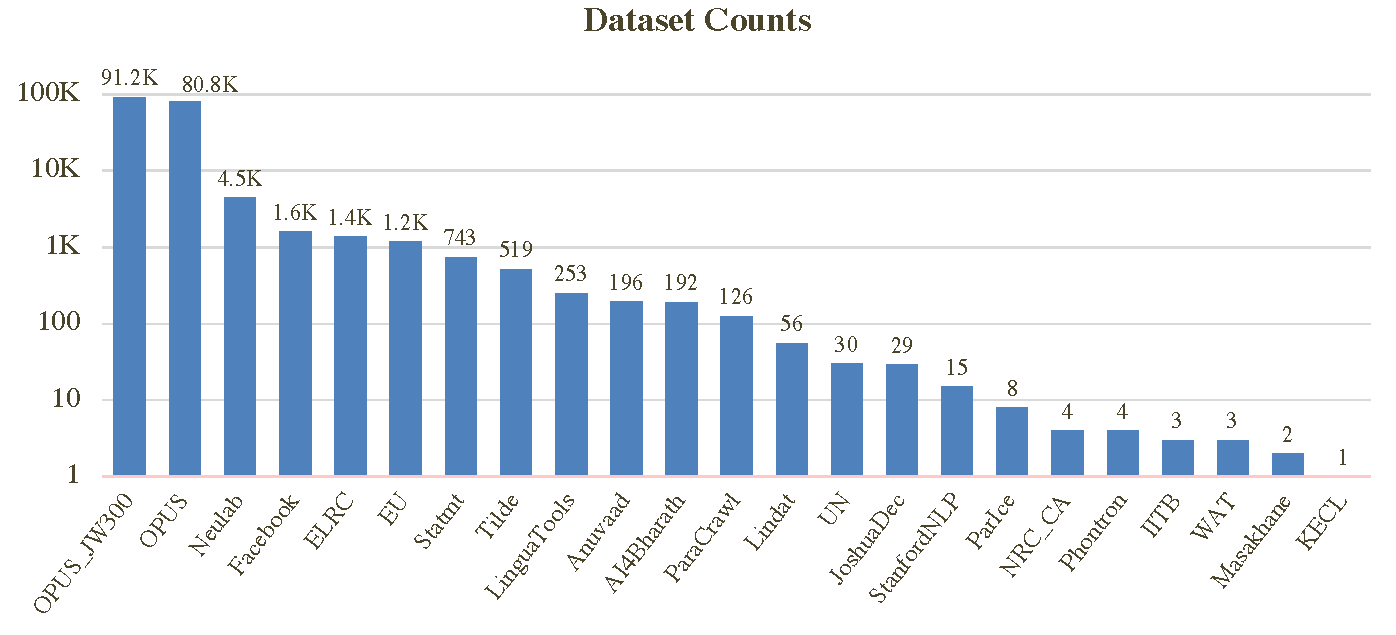
\includegraphics[width=\linewidth]{img/manyeng/mtdata-stats.pdf}
    \caption{Datasets curated from various sources. These statistics are extracted as of 2022 February (version 0.3.4)}.
    \label{fig:mtdata-stats}
\end{figure}


\begin{comment}
%\begin{figure*}[ht]
\begin{sidewaysfigure}
\centering
    %trim={5mm 4mm 5mm 5mm},clip
    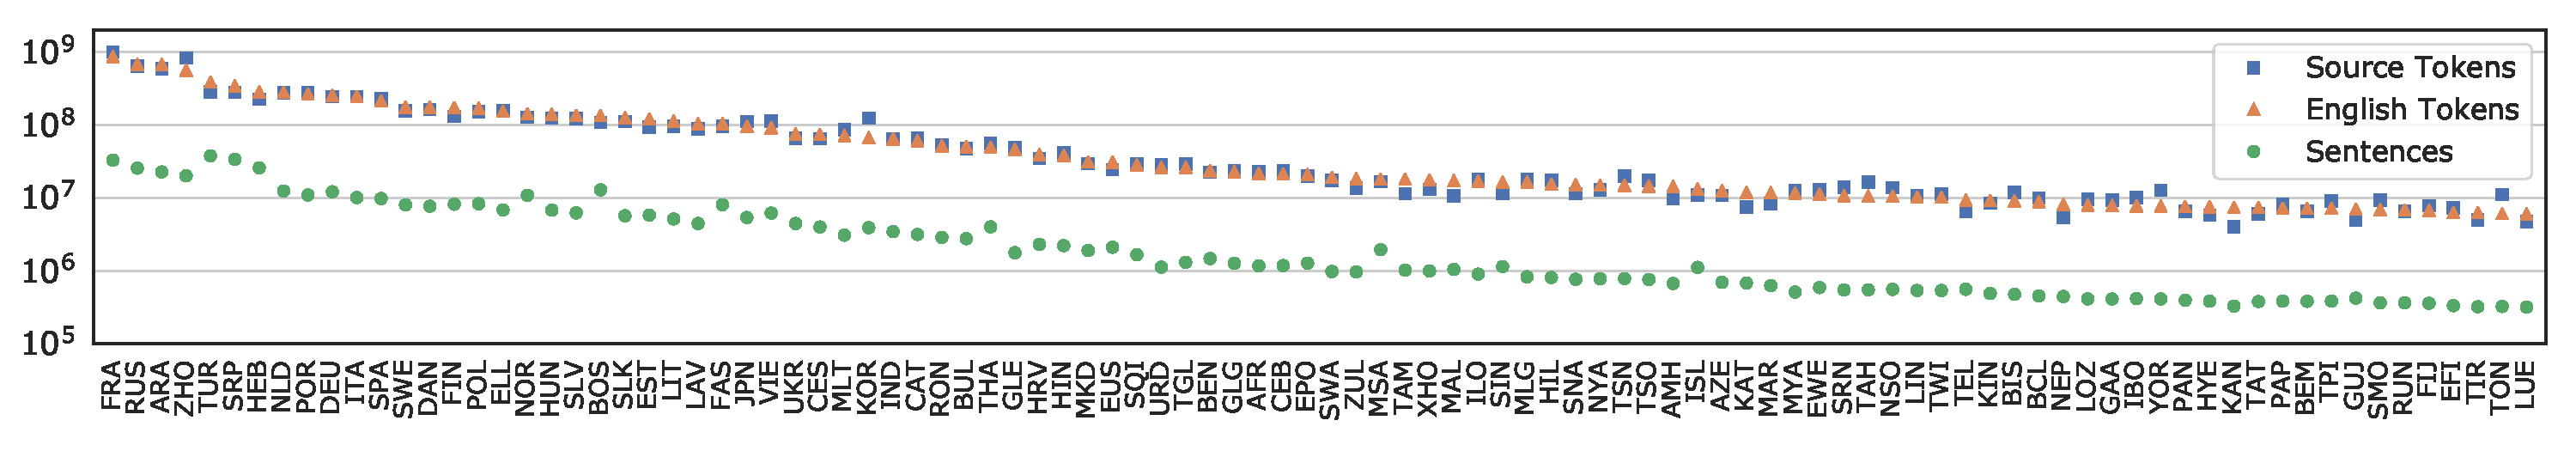
\includegraphics[height=0.14\vsize,trim={5mm 4mm 5mm 5mm},clip]{manyeng/lang-stats-1-100.pdf}
    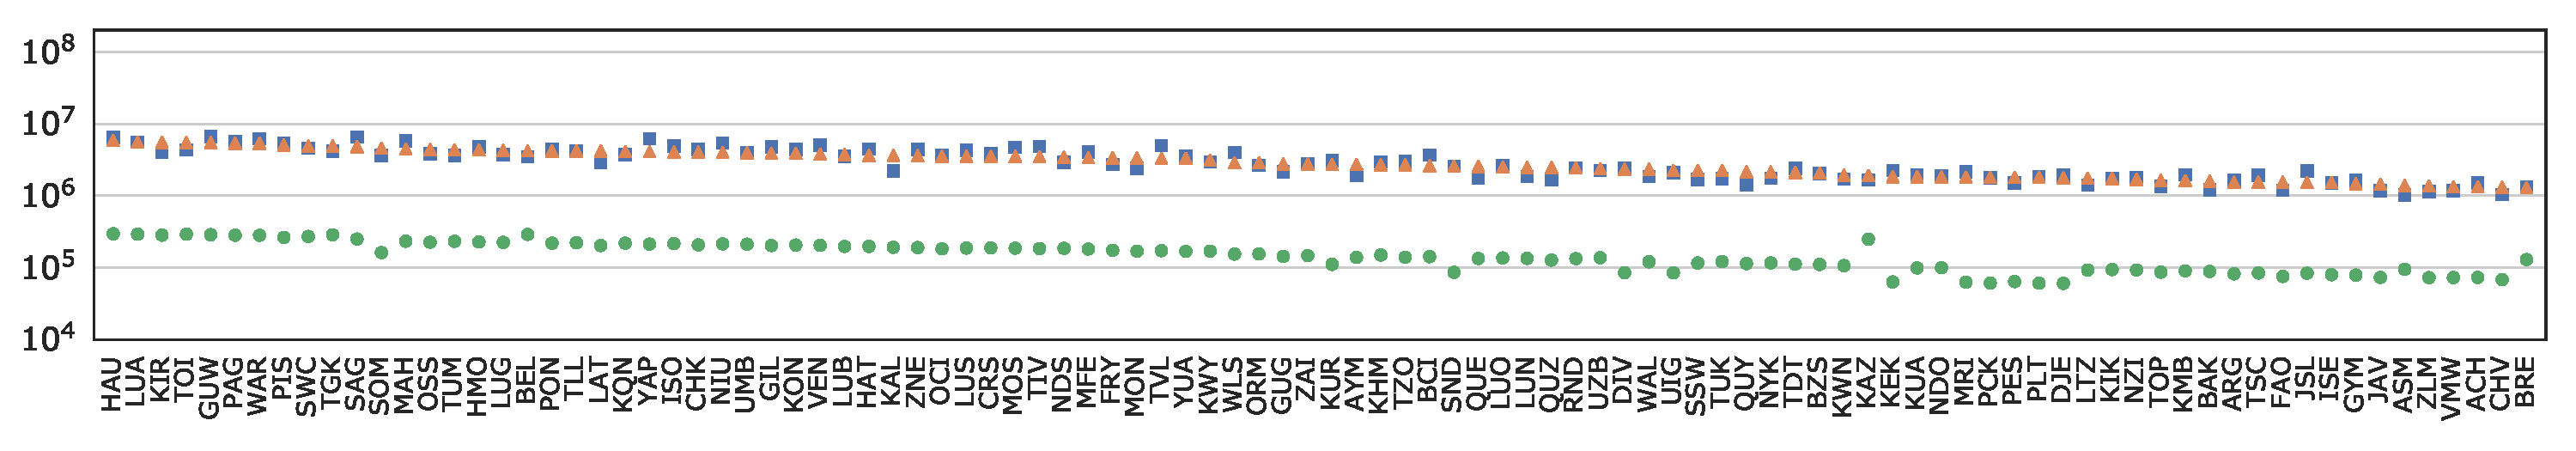
\includegraphics[height=0.14\vsize,trim={5mm 4mm 5mm 5mm},clip]{manyeng/lang-stats-101-200.pdf}
    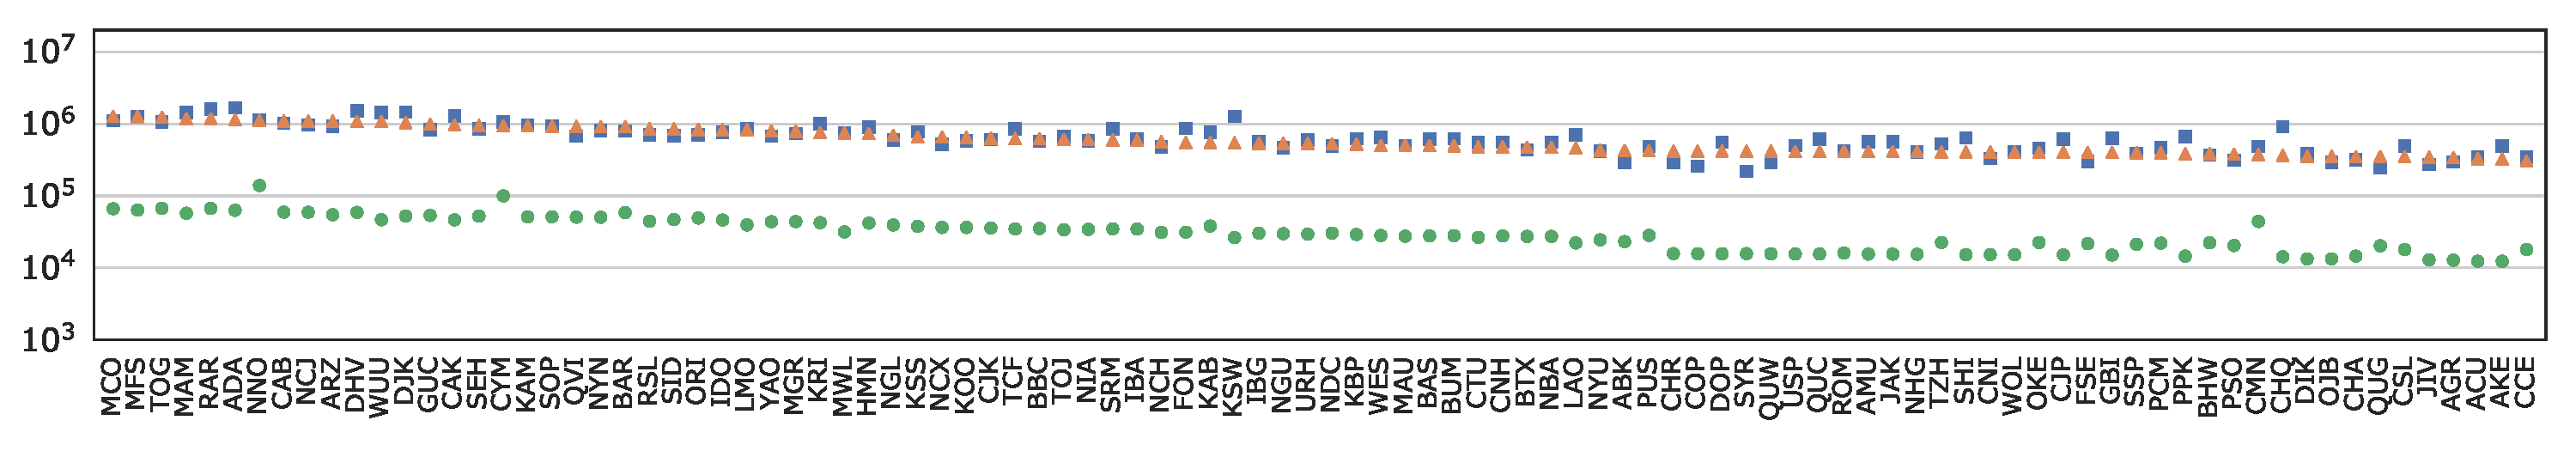
\includegraphics[height=0.14\vsize,trim={5mm 4mm 5mm 5mm},clip]{manyeng/lang-stats-201-300.pdf}
    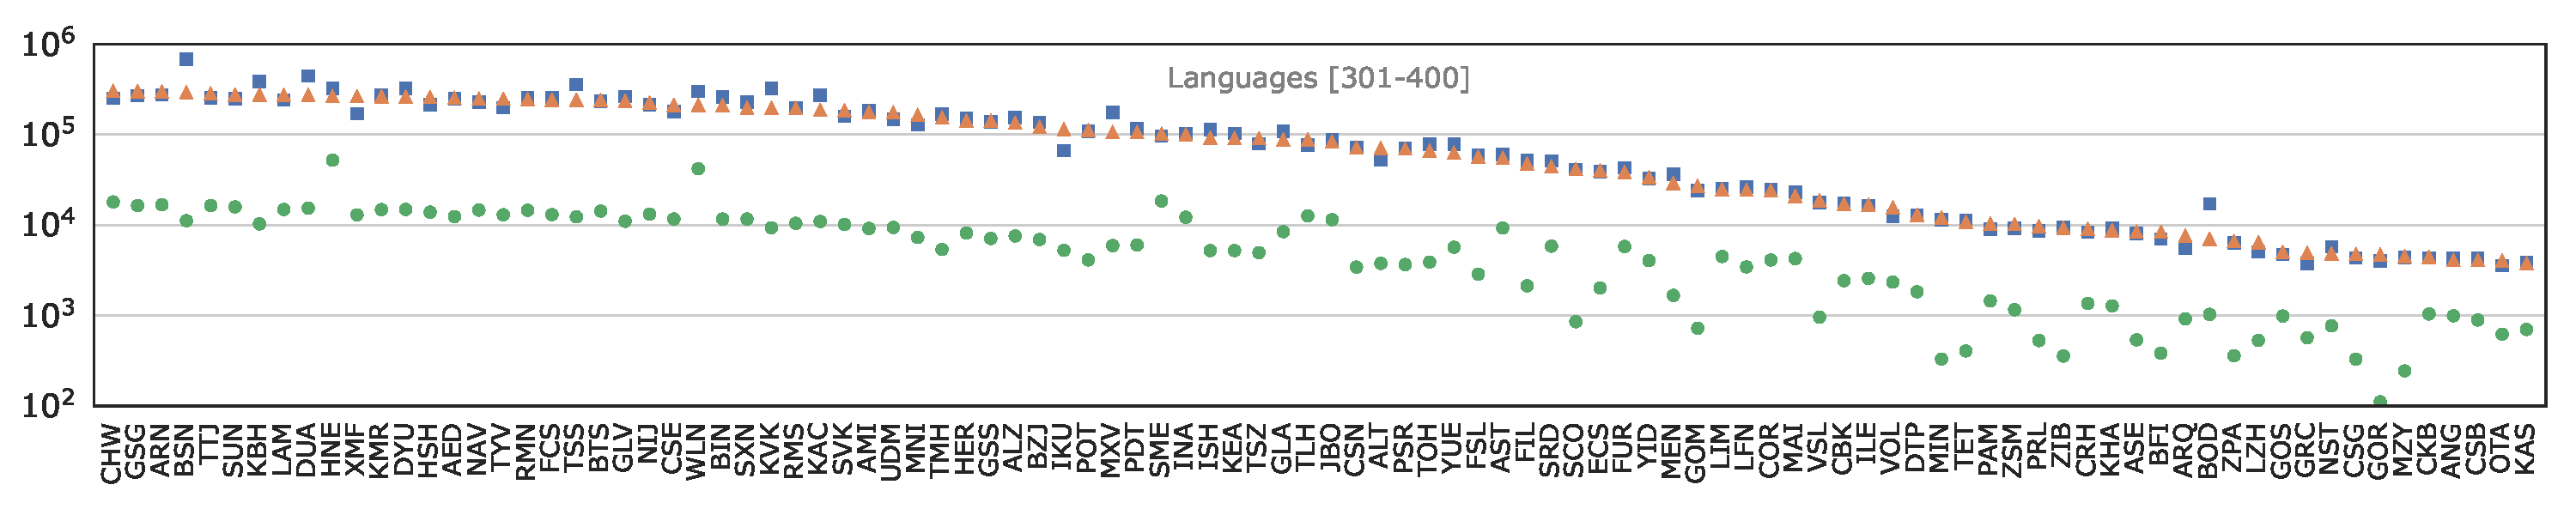
\includegraphics[height=0.14\vsize,trim={5mm 4mm 5mm 5mm},clip]{manyeng/lang-stats-301-400.pdf}
    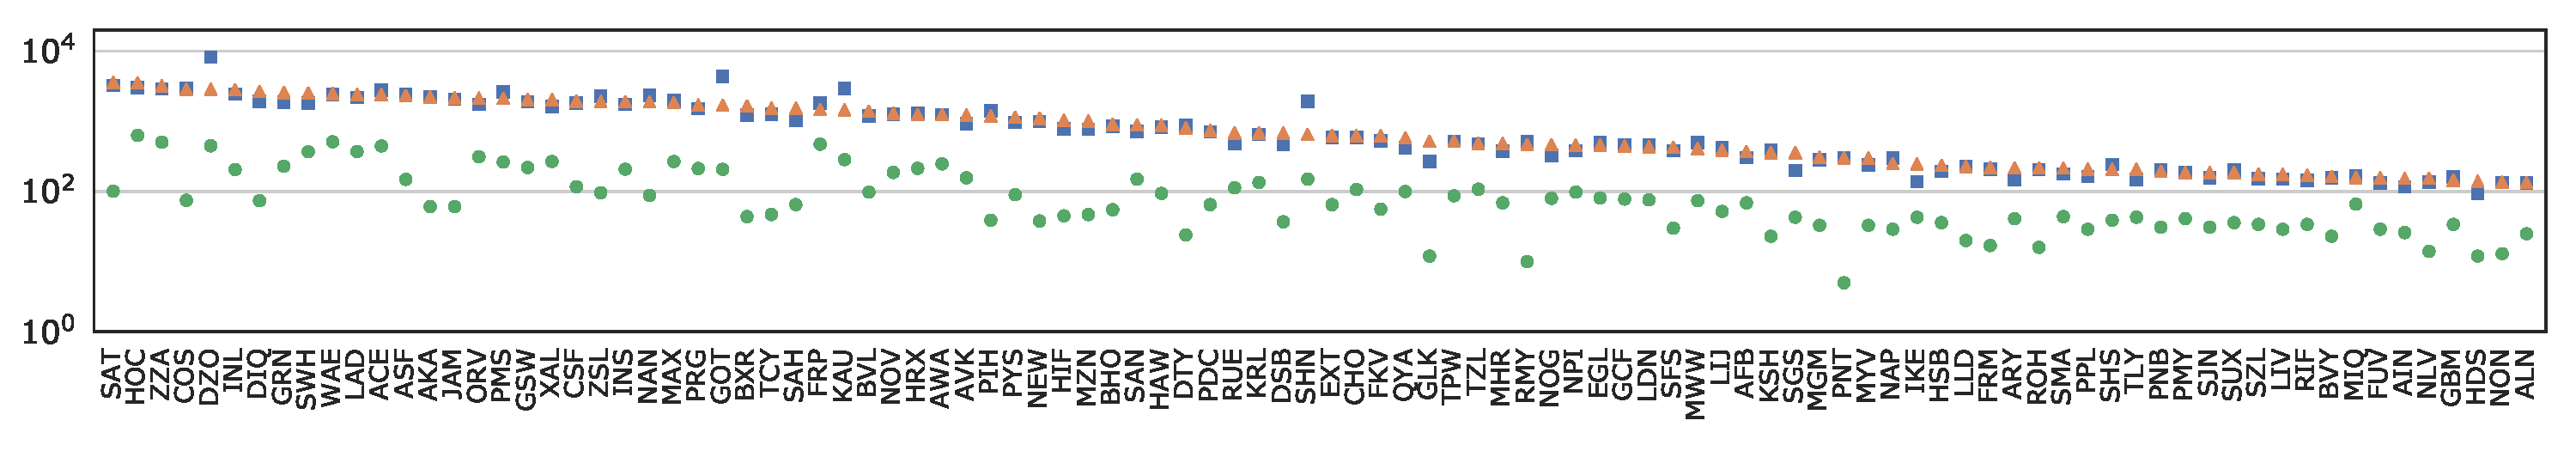
\includegraphics[height=0.14\vsize,trim={5mm 4mm 5mm 5mm},clip]{manyeng/lang-stats-401-500.pdf}     
    \caption{\centering Training data statistics for 500 languages, sorted as descending order of English token count,  obtained after de-duplication and filtering (see Section~\ref{sec:datasets}). The full name for these ISO 639-3 codes can be looked up using \mtdata, e.g. \texttt{mtdata-iso eng}. }
       \label{fig:train-data-stats}
\end{sidewaysfigure}
%\end{figure*}
\end{comment}

\begin{figure*}[h!t]
\centering
    %trim={5mm 4mm 5mm 5mm},clip
    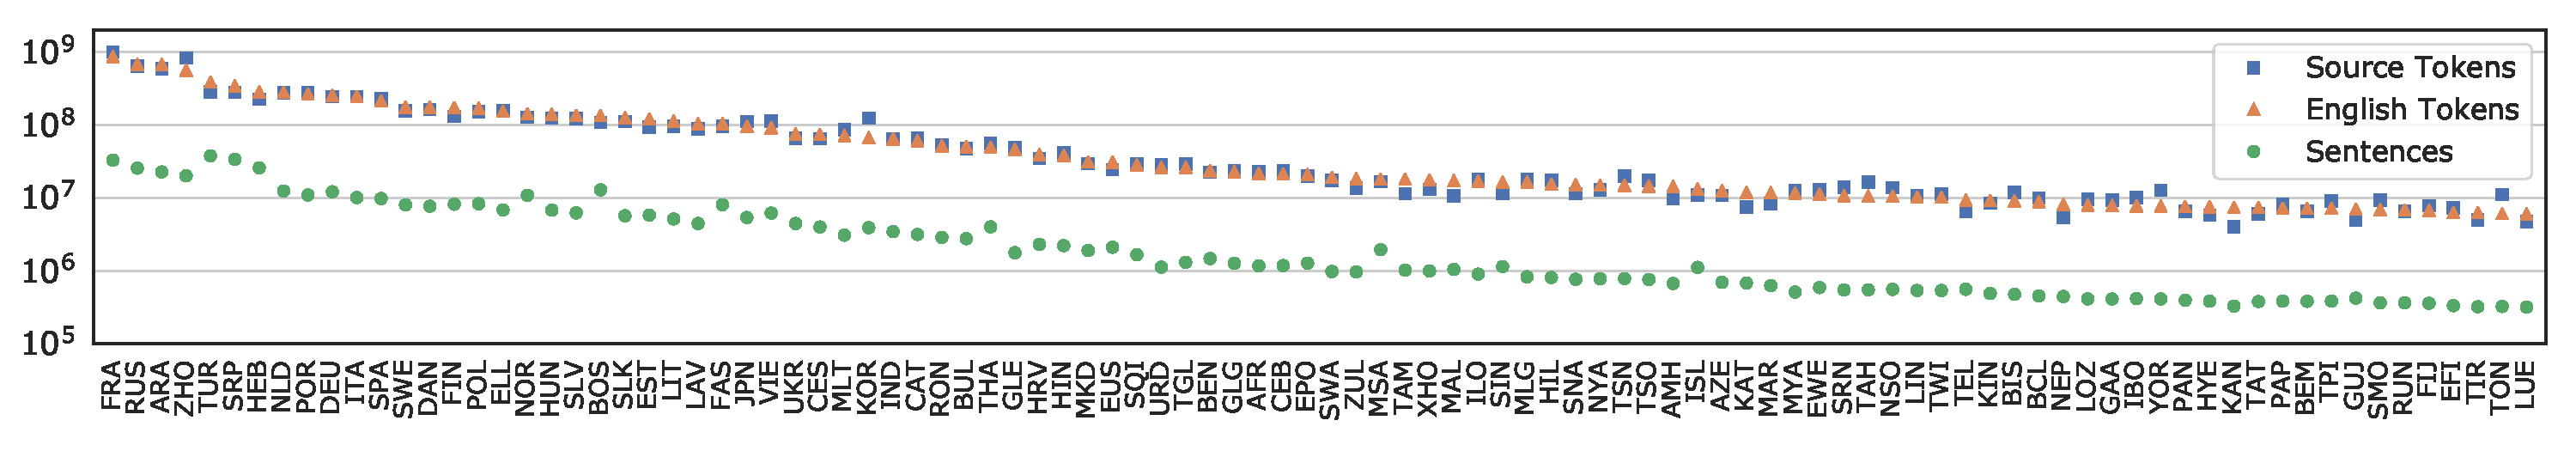
\includegraphics[width=\linewidth,trim={5mm 4mm 5mm 5mm},clip]{manyeng/lang-stats-1-100.pdf}
    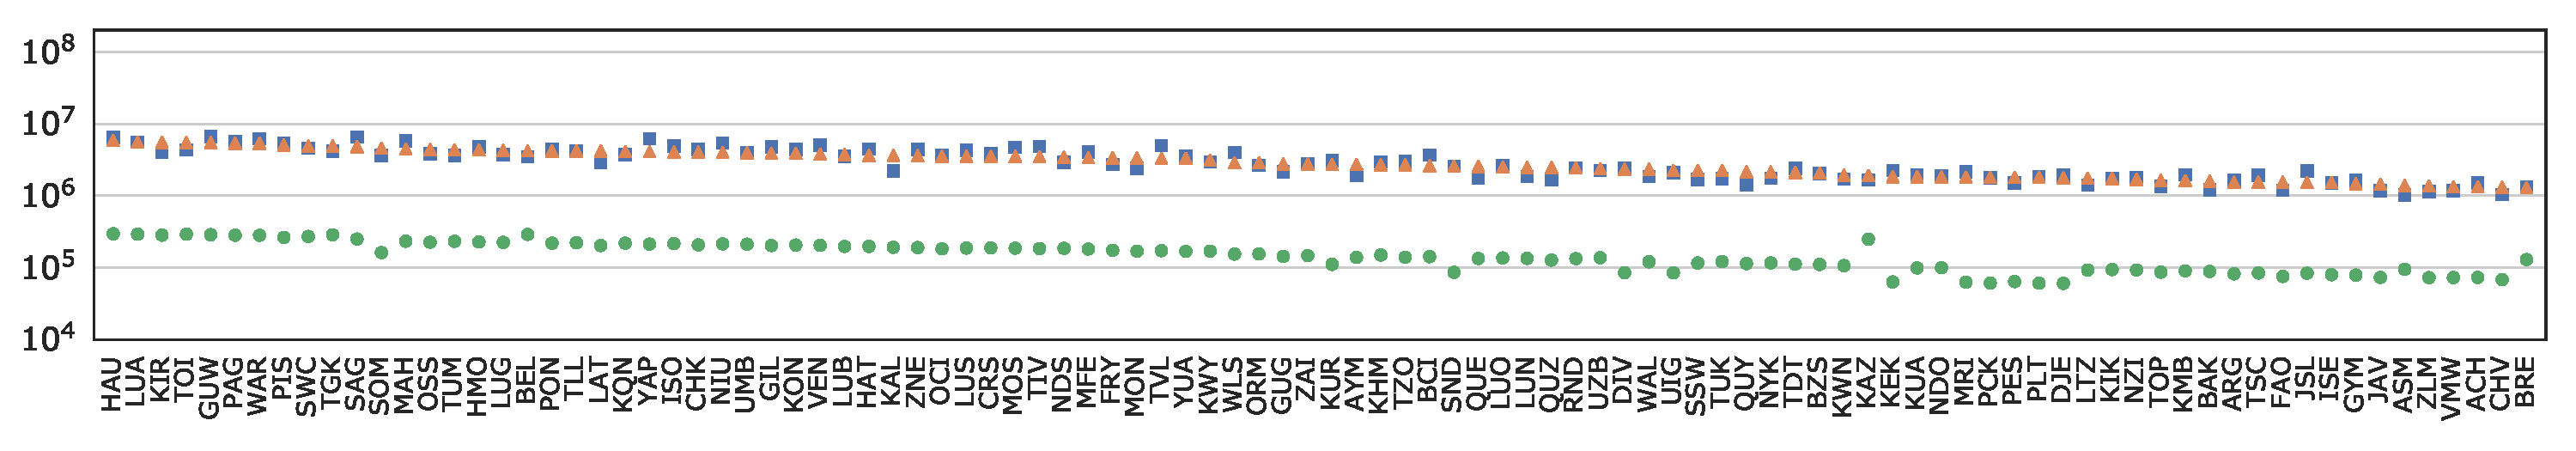
\includegraphics[width=\linewidth,trim={5mm 4mm 5mm 5mm},clip]{manyeng/lang-stats-101-200.pdf}
    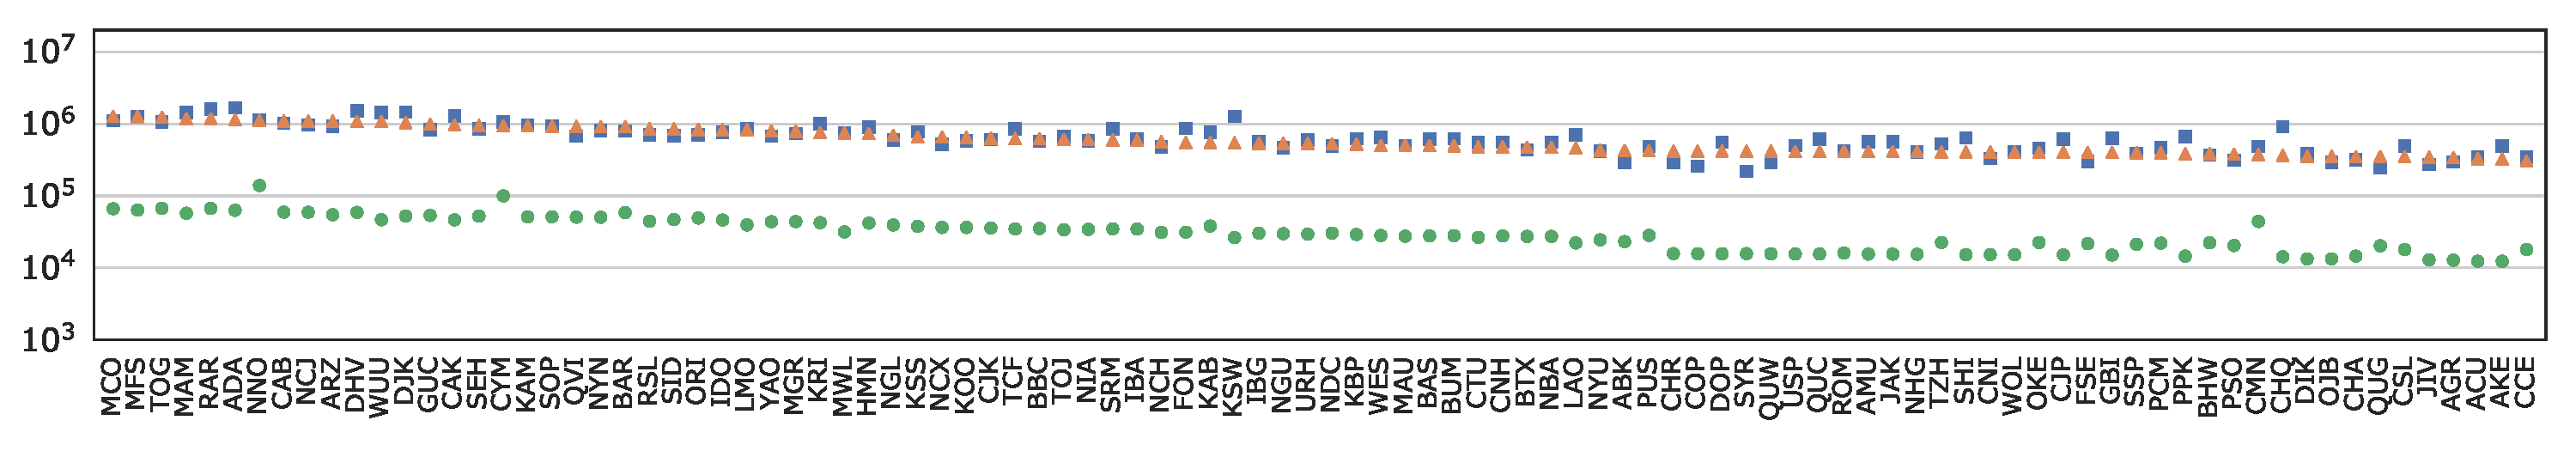
\includegraphics[width=\linewidth,trim={5mm 4mm 5mm 5mm},clip]{manyeng/lang-stats-201-300.pdf}
    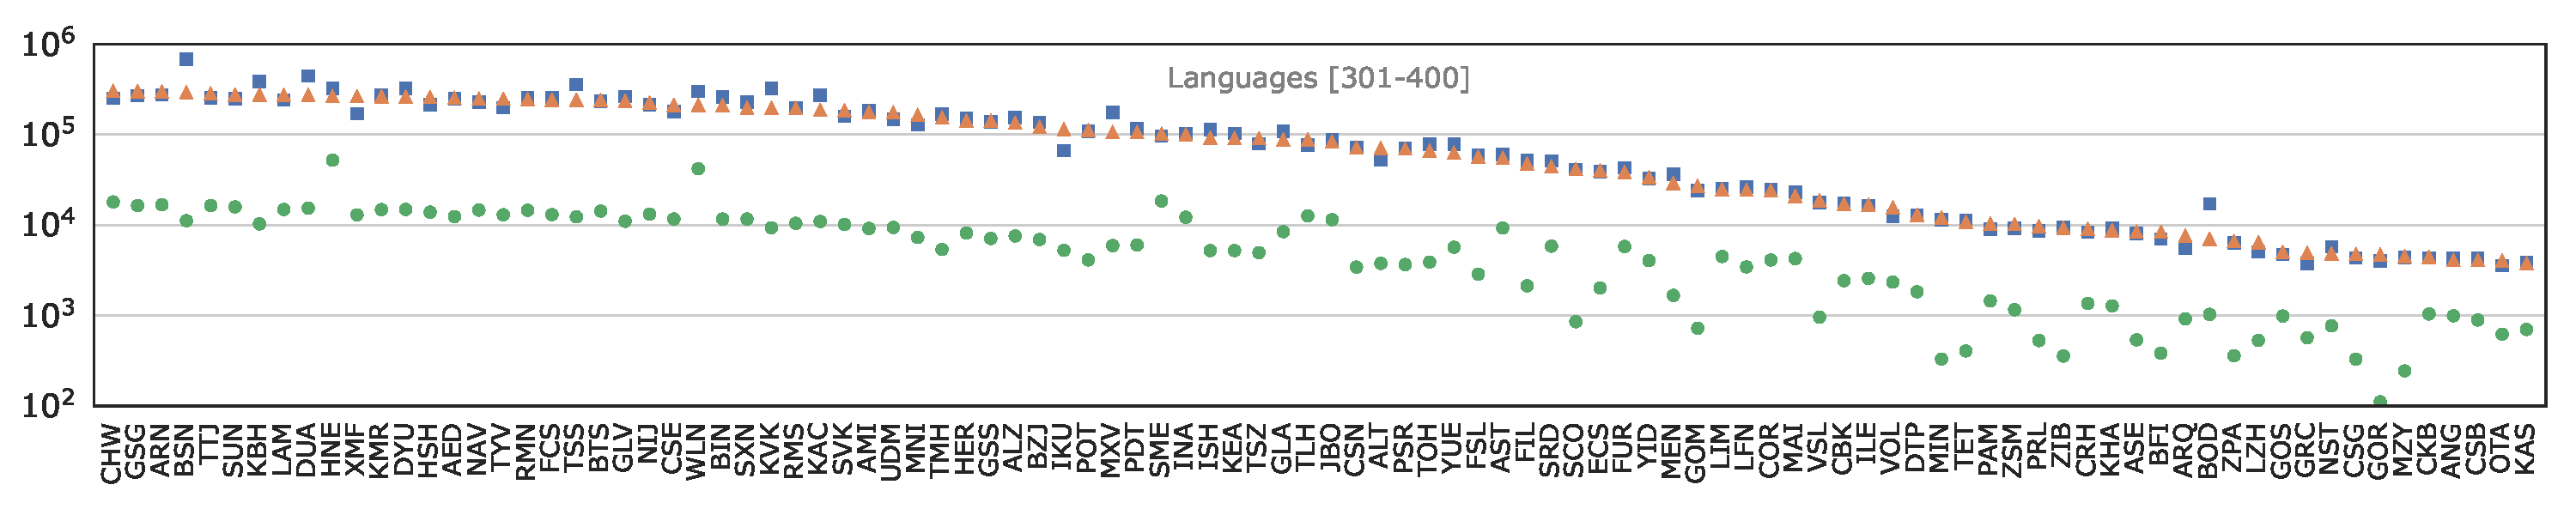
\includegraphics[width=\linewidth,trim={5mm 4mm 5mm 5mm},clip]{manyeng/lang-stats-301-400.pdf}
    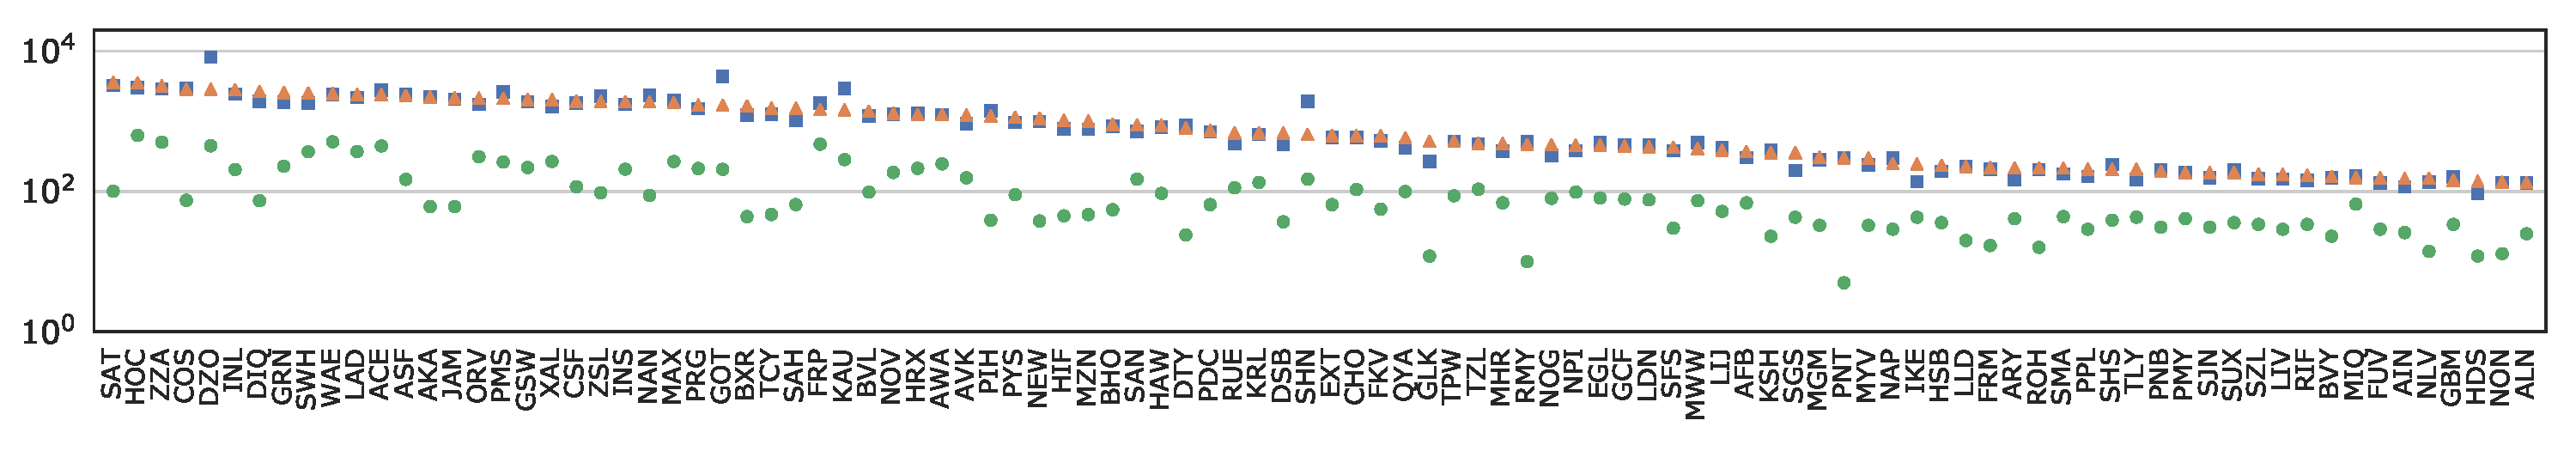
\includegraphics[width=\linewidth,trim={5mm 4mm 5mm 5mm},clip]{manyeng/lang-stats-401-500.pdf}     
    \caption{Training data statistics for 500 languages, sorted as descending order of English token count,  obtained after deduplication and filtering (see Section~\ref{sec:datasets}). The full name for these ISO 639-3 codes can be looked up using \mtdata, e.g. \texttt{mtdata-iso eng}.}
       \label{fig:train-data-stats}
\end{figure*}



\textbf{Cleaning:}
 We use \textsc{SacreMoses}\footnote{\url{https://github.com/isi-nlp/sacremoses} a fork of \url{https://github.com/alvations/sacremoses} with improvements to tokenization for many low resource languages.} to normalize Unicode punctuations and digits, followed by word tokenization. 
We remove records that are duplicates, have abnormal source-to-target length ratios, have many non-ASCII characters on the English side, have a URL, or which overlap exactly, either on the source or target side, with any sentences in held out sets.
As preprocessing is compute-intensive, we parallelize using Apache Spark.
The cleaning and tokenization results in a corpus of 474 million sentences and 9 billion tokens on the source and English sides each. The token and sentence count for each language are provided in Figure~\ref{fig:train-data-stats}.
Both the processed and raw datasets are available at \url{http://rtg.isi.edu/many-eng/data/v1/}.\footnote{A copy is at \url{https://opus.nlpl.eu/MT560.php}}

\subsection{Many-to-English Multilingual Model}
\label{sec:500eng-model}
We use \rtg\ to train Transformer NMT \cite{vaswani-2017-attention} with a few modifications.
Firstly, instead of a shared BPE vocabulary for both source and target, we use two separate BPE vocabularies. 
Since the source side has 500 languages and the target side has English only, we use a large source vocabulary and a relatively smaller target vocabulary.
A larger target vocabulary leads to higher time and memory complexity, whereas a large source vocabulary increases only the memory complexity but not the time complexity.
We train several models, ranging from the standard 6 layers, 512-dimensional Transformers to larger ones with more parameters. Since the dataset is massive, a larger model trained on big mini-batches yields the best results. Our best performing model is a 768 dimensional model with 12 attention heads, 9 encoder layers, 6 decoder layers, feed-forward dimension of 2048, dropout and label smoothing at 0.1, using $512,000$ and $64,000$ BPE types as source and target vocabularies, respectively. The decoder's input and output embeddings are shared.
Since some English sentences are replicated to align with many sentences from different languages (e.g. the Bible corpus), BPE merges are learned from the deduplicated sentences using \nlcodec.
Our best performing model is trained with an effective batch size of about 720,000 tokens per optimizer step. Such big batches are achieved by using mixed-precision distributed training on 8 NVIDIA A100 GPUs with gradient accumulation of 5 mini-batches, each having a maximum of 18,000 tokens. We use the Adam optimizer~\cite{kingma2015adam} with 8000 warm-up steps followed by a decaying learning rate, similar to \citet{vaswani-2017-attention}. 
We stop training after five days and six hours when a total of 200K updates are made by the optimizer; validation loss is still decreasing at this point. 
To assess the translation quality of our model, we report BLEU~\cite{papineni-etal-2002-bleu,post-2018-sacrebleu}\footnote{All our BLEU scores are obtained from \sacrebleu\ \texttt{BLEU+c.mixed+\#.1+s.exp+tok.13a+v.1.4.13}.} on a subset of languages for which known test sets are available, as given in Figure~\ref{fig:test-bleu}, along with a comparison to \citet{zhang-etal-2020-multiling-nmt}'s best model.\footnote{
%a multilingual 24-layered 512-dimensional Transformer model having Merged Attention, Language-aware Layer Normalization and Linear Transformation, and trained including random online backtranslation.
Scores are obtained from \url{https://github.com/bzhangGo/zero/tree/master/docs/multilingual_laln_lalt}; accessed: 2021/03/30}

\begin{figure*}[ht]
    \centering
    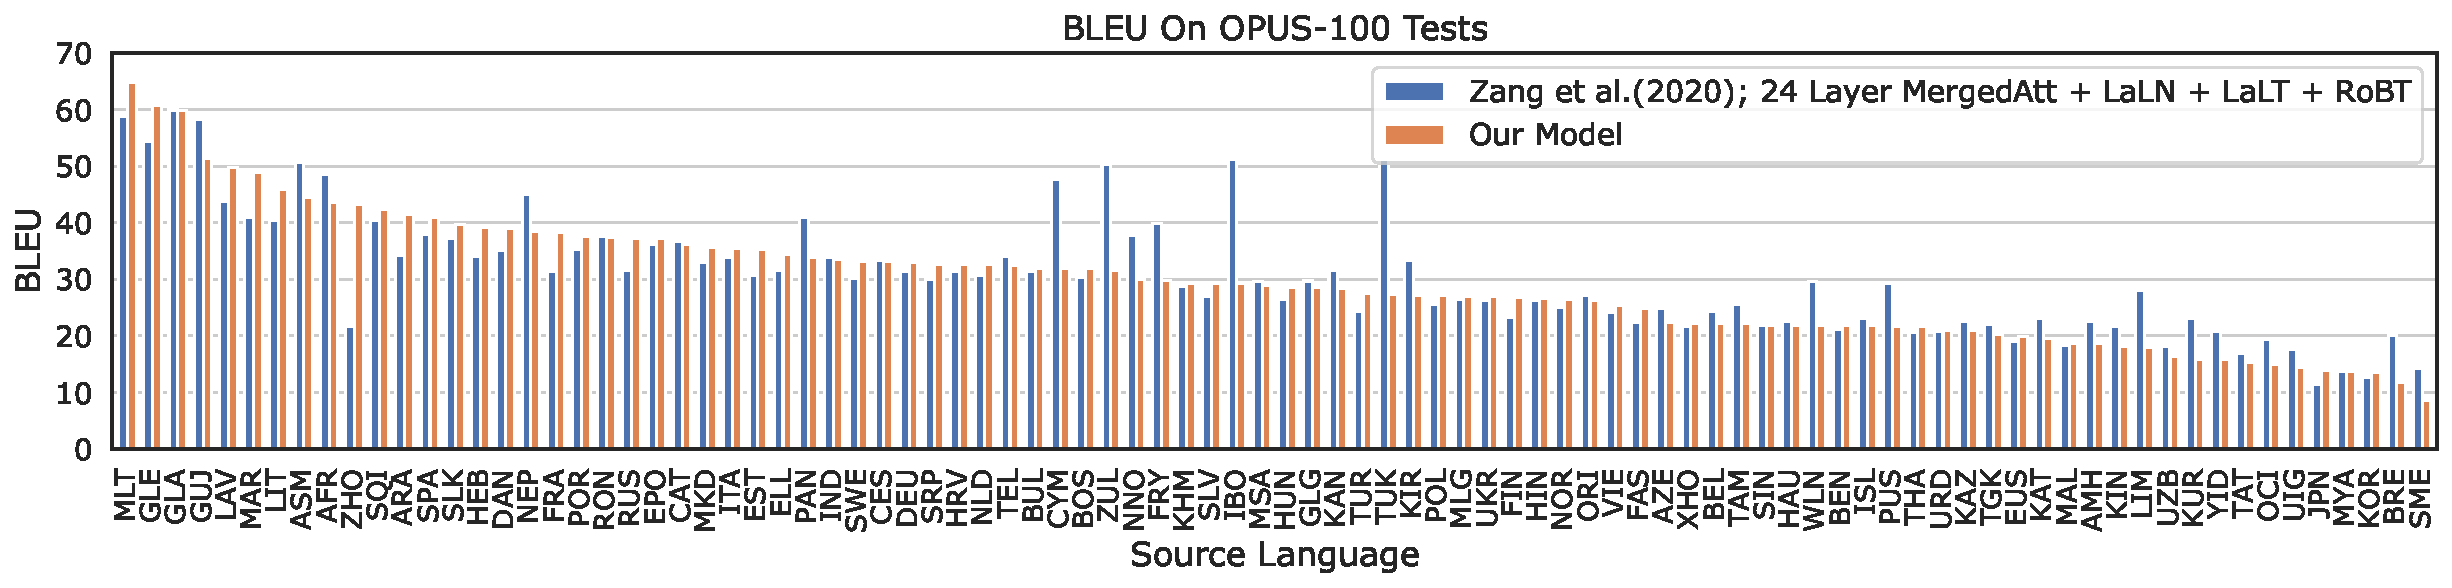
\includegraphics[width=1\textwidth]{manyeng/BLEU-opus100.pdf}
    \caption[Many-to-English model's BLEU scores on OPUS-100 test set]{Many-to-English BLEU on OPUS-100 tests~\cite{zhang-etal-2020-multiling-nmt}. 
    Despite having four times more languages on the source side, our model scores competitive BLEU on most languages with the strongest system of \citet{zhang-etal-2020-multiling-nmt}. The tests where our model scores lower BLEU have shorter source sentences (mean length of about three tokens).}
    \label{fig:test-bleu}
\end{figure*}
%All BLEU scores are mixed-cased and are obtained using the default settings of \sacrebleu.
% https://github.com/bzhangGo/zero/tree/master/docs/multilingual_laln_lalt

\begin{comment}
\begin{subfigure}[t]{0.68\textwidth}
        \centering
        \includegraphics[width=\linewidth]{manyeng/BLEU-nttalksv1.pdf}
        %\caption{Lorem ipsum}
    \end{subfigure}%
    ~ 
    \begin{subfigure}[t]{0.31\textwidth}
        \centering
        \includegraphics[width=\linewidth,trim={7mm 0mm 0mm 0mm},clip]{img/BLEU-wmt-etc.pdf}
        %\caption{Lorem ipsum}
    \end{subfigure}
     TED Talks~\cite{qi-etal-2018-pretrainemb}, WMT~\cite{barrault-etal-2019-findings}, UNv1~\cite{ziemski-etal-2016-unpc}, and Indian-6~\cite{post-etal-2012-constructing}.
\end{comment}



\section{Applications}
\label{sec:value}
The model we trained as a demonstration for our tools is useful on its own, as described in the following sections. 

\subsection{Readily Usable Translation Service}
\label{sec:value.off-shelf-mt}
Our pretrained NMT model is readily usable as a service capable of translating several hundred source languages to English.
By design, source language identification is not necessary.
Figure~\ref{fig:test-bleu} shows that the model scores more than 20 BLEU, which maybe be a useful quality for certain downstream applications involving web and social media content analysis.
Apache Tika \cite{mattmann2011tika}, a content detection and analysis toolkit capable of parsing thousands of file formats, has an option for translating any document into English using our multilingual NMT model.\footnote{\url{https://cwiki.apache.org/confluence/display/TIKA/NMT-RTG}} Our model has been packaged and published to DockerHub\footnote{\url{https://hub.docker.com/}}, which can be obtained by the following command:
\begin{minted}[
%frame=lines,
%framesep=2mm,
baselinestretch=1.1,
fontsize=\normalsize,
%linenos
]{bash}
docker run --rm -i -p 6060:6060 tgowda/rtg-model:500toEng-v1
# For GPU backend, add --gpus '"device=0"' 
\end{minted}

The above command starts a docker image with HTTP server having a web interface, as can be seen in Figure~\ref{fig:rtg-webui}, and a REST API.
An example interaction with the REST API is as follows: 
\begin{figure}[ht]
    \centering
    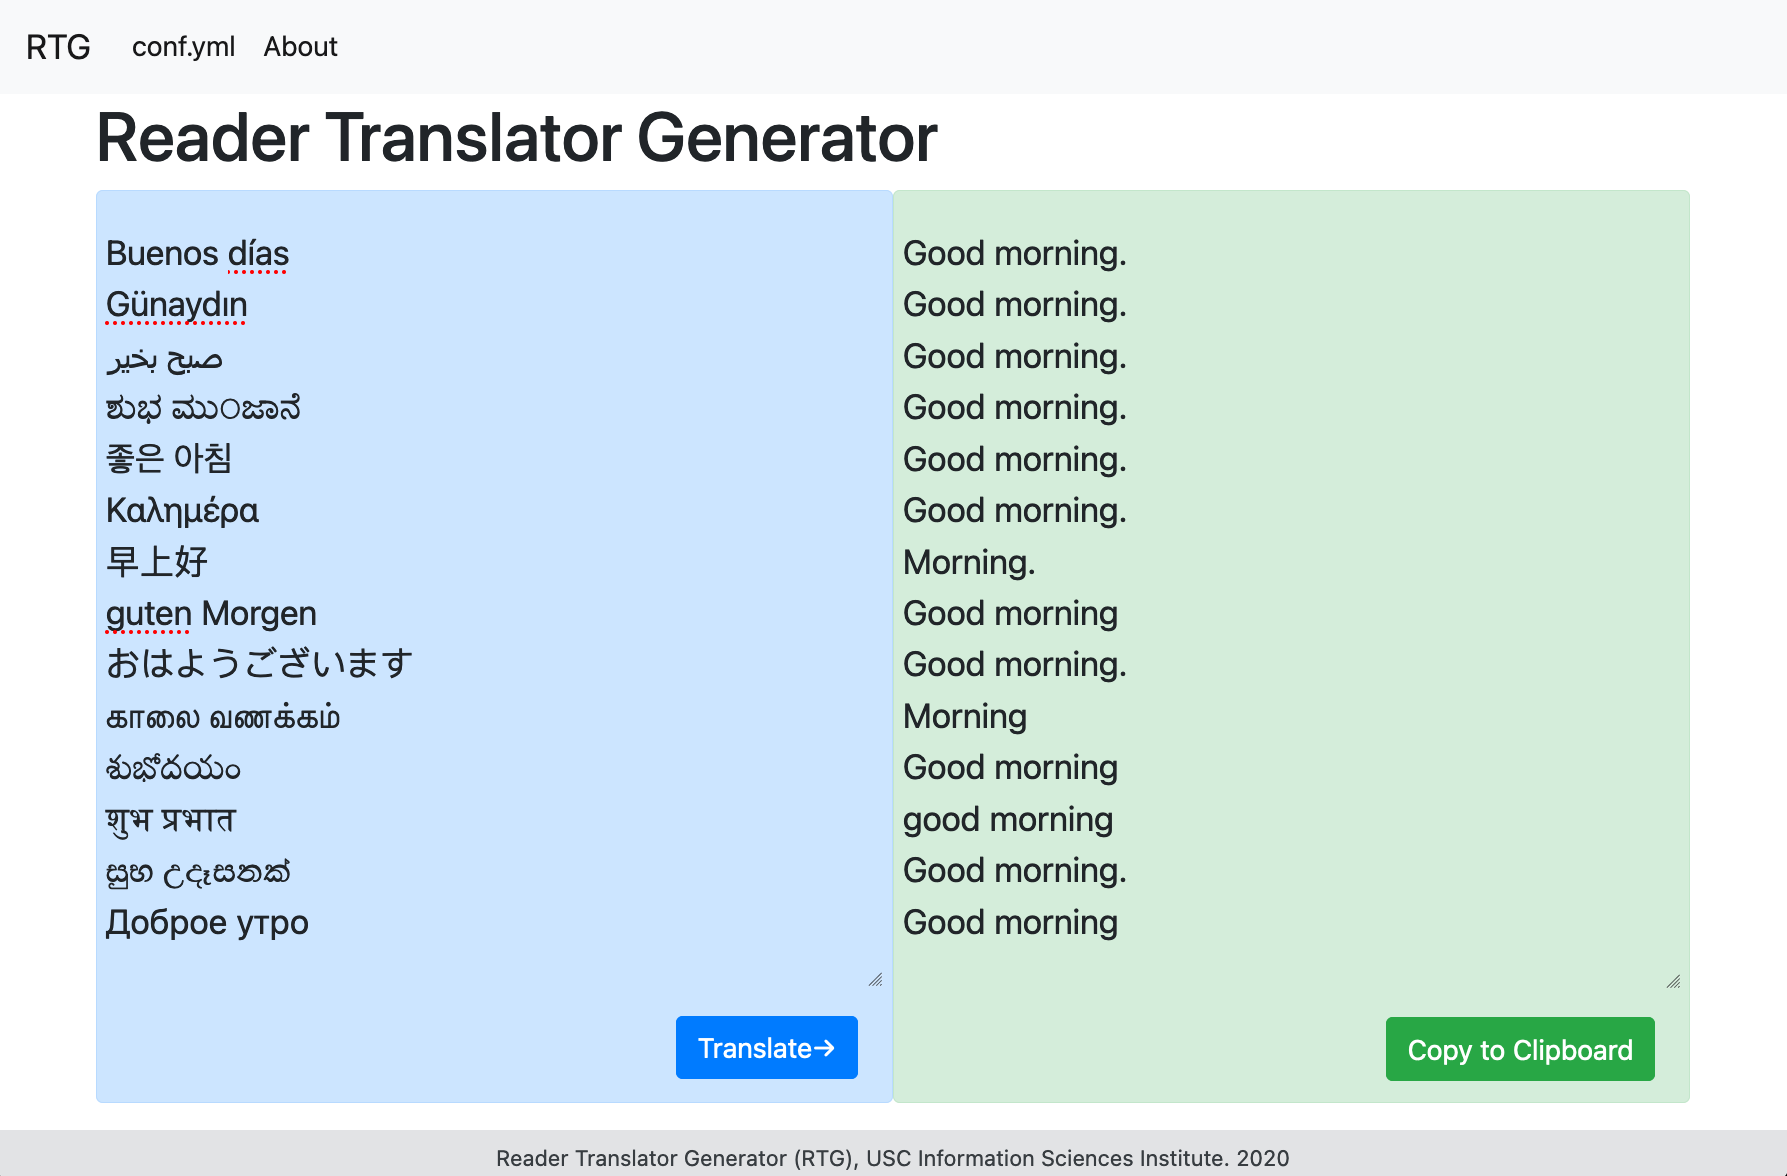
\includegraphics[width=0.8\linewidth,trim=20 60 100 15,clip]{manyeng/rtg-webui.png}
    \caption{RTG Web Interface}
    \label{fig:rtg-webui}
\end{figure}

\begin{minted}[baselinestretch=1.1, fontsize=\normalsize]{bash}
$ API="http://localhost:6060/translate"
$ curl --data "source=Comment allez-vous?" --data "source=Bonne journée" $API
\end{minted}

\begin{minted}[baselinestretch=1.1, fontsize=\normalsize]{json}
 { 
   "source": [ "Comment allez-vous?", "Bonne journée" ],
   "translation": [ "How are you?", "Have a nice day" ]
}
\end{minted}


\subsection{Parent Model for Low Resource MT}
\label{sec:value.transfer-learning}
%WMT 20 has two low resource languages: IU and KM http://statmt.org/wmt20/translation-task.html 
%Uyghur from Lorelei?  Pashto  from Material?
 Fine-tuning is a useful transfer learning technique for improving the translation of low resource languages ~\cite{zoph-etal-2016-transfer,neubig-hu-2018-rapid,gheini2019universal}. 
 In the following subsections, we explore fine-tuning in both bilingual and multilingual setups.
 
 \subsubsection{Bilingual Setup}
Consider Breton-English (bre-eng) and Northern Sami-English (sme-eng), two of the low resource settings for which our model has relatively low BLEU (see Figure~\ref{fig:test-bleu}). 
To show the utility of fine-tuning with our model, we train a strong baseline Transformer model, one for each language, from scratch using OPUS-100 training data~\cite{zhang-etal-2020-multiling-nmt}, and fine-tune our multilingual model on the same dataset as the baselines. We shrink the parent model vocabulary and embeddings to the child model dataset, and train all models on NVIDIA P100 GPUs until convergence.\footnote{More info: \url{https://github.com/thammegowda/006-many-to-eng/tree/master/lowres-xfer}}
 Table~\ref{tab:transfer-lowres}, which shows BLEU on the OPUS-100 test set for the two low resource languages, indicates that our multilingual NMT parent model can be further improved with fine-tuning on limited training data.
 The fine-tuned model achieves 10 \bleu{} higher than the baseline model.

\begin{table}[ht]
    \centering
    %\footnotesize
    \begin{tabular}{l  r r}
        Model     & bre-eng & sme-eng \\ \hline\hline
        Baseline  & 12.7  &  10.7  \\
        Parent    & 11.8  &  8.6  \\
        \textit{Finetuned} & \textbf{22.8}  & \textbf{19.1}  \\ 
    \end{tabular}
    \caption{Finetuning our multilingual NMT on limited training data in low resource settings significantly improves translation quality, as quantified by BLEU.}
    \label{tab:transfer-lowres}
\end{table}

\subsubsection{Multilingual Model}
In the previous section, the 500-English multilingual model was proven effective while independently adapting to each rare language, e.g., bre-eng and sme-eng. 
In this section, we explore joint adaptation simultaneously to 9 low resource languages, taken from IARPA MATERIAL program.\footnote{https://www.iarpa.gov/research-programs/material}.
Table~\ref{tab:material-lang-stats} provides training data statistics for all nine languages. 
See Table \ref{tab:material-scores} for the results.

\begin{table}[h!t]
\small
\centering
\begin{tabular}{l | rrr | rrr} 
\hline 
\multirow{2}{*}{ Languages } & \multicolumn{3}{c |}{Clean parallel} & \multicolumn{3}{c}{Noisy parallel} \\
& Sents & Source Toks & English Toks & Sents & Source Toks & English Toks \\ \hline \hline 
swa-eng & 72.3k & 1.8M & 2.0M & 498k & 12.6M & 14.8M \\
tgl-eng & 46.7k & 804k & 823k & 744k & 21.4M & 20.7M \\
som-eng & 21.5k & 651k & 688k & 4.8M & 124.0M & 126.3M \\
lit-eng & 39.5k & 655k & 857k & 3.0M & 64.1M & 76.0M \\
pus-eng & 39.9k & 886k & 820k & 1.05M & 14.2M & 12.9M \\
bul-eng & 38.1k & 773k & 858k & 11.1M & 282.4M & 295.2M \\
kat-eng & 3.3k & 52k & 74k & 3.5M & 59.0M & 76.1M \\
kaz-eng & 71.4k & 559k & 595k & 25.0M & 423M & 515.9M \\
fas-eng & 31.7k & 715k & 798k & 249k & 5.6M & 5.3M \\ \hdashline
Combined & 364.3k & 6.9M & 7.5M & 49.9M & 1.0B & 1.1B \\
\hline 
\end{tabular} 
\caption{Training data statistics for 9 low resource languages used in IARPA MATERIAL program.}
\label{tab:material-lang-stats}
\end{table}

%\vspace{6mm}

\begin{table}
\small 
\centering
    \begin{tabular}{l | rrrr | rrrr}
    \hline
& \multicolumn{4}{c|}{BLEU (lc detok) on Analysis} & \multicolumn{4}{c}{MacroF1 (lc detok) on Analysis} \\
Languages & Prev best & 500-Eng & +ft.noisy & +ft.clean & Prev best & 500-Eng & +ft.noisy & +ft.clean \\ \hline \hline
swa-eng & 34.4 & 26.6 & 36.0 & \textbf{38.3} & 35.7 & 29.8 & 37.5 & \textbf{39.2} \\
tgl-eng & 39.5 & 33.5 & 40.7 & \textbf{43.3} & 45.0 & 40.9 & \textbf{48.1} & 47.5 \\
som-eng & 24.4 & 7.7 & 24.9 & \textbf{27.7} & 26.2 & 10.8 & 28.0 & \textbf{30.0} \\
lit-eng & 32.6 & 25.1 & 33.1 & \textbf{35.4} & \textbf{39.4} & 26.7 & 37.6 & 37.2 \\
pus-eng & 20.9 & 5.9 & 20.4 & \textbf{21.9} & 19.2 & 8.2 & 20.1 & \textbf{21.1} \\
bul-eng & 45.2 & 39.3 & 44.9 & \textbf{48.2} & \textbf{46.5} & 41.0 & 45.2 & 43.5 \\
kat-eng & 31.9 & 21.2 & \textbf{32.2} & 30.1 & 32.7 & 19.9 & \textbf{34.3} & 29.5 \\
kaz-eng & \textbf{30.4} & 15.2 & 27.0 & 25.6 & 26.4 & 15.0 & \textbf{26.2} & 23.4 \\
fas-eng & 27.2 & 21.8 & 27.1 & \textbf{28.3} & 23.9 & 22.3 & \textbf{25.3} & 23.7 \\ \hline
\end{tabular} 
    \caption[Multilingual NMT achieves state-of-the-art performance on low resource language via finetuning]{Multilingual NMT achieves state-of-the-art performance on low resource language via finetuning. \textit{`Prev best'} is the best performing bilingual model (1 per each setting). \textit{`+ft.noisy'} is 500-eng model finetuned to noisy parallel data, and \textit{`+ft.clean'} is \textit{`+ft.noisy'} further finetuned on a limited quantity of clean parallel data (see Table~\ref{tab:material-lang-stats}). }
    \label{tab:material-scores}
\end{table}


\subsection{Cross-lingual Contextual Embeddings}

The multilingual NMT model's encoder learns bi-directional contexualized embeddings that are cross-lingual across 500 languages.
We created a sequence classifier, and initialized the source embeddings matrix and all the encoder layers from our multilignual NMT. 
We fine-tuned the classifier on MultiNLI~\cite{williams-etal-2018-multinli} dataset with English training data, and evaluated on XNLI datasets on 15 languages~\cite{conneau-etal-2018-xnli}. 
This setup commonly known as ``zero-shot transfer'' or "cross-lingual transfer" in literature. 
During the fine-tuning, embeddings and all other parameters, except the last layer, were frozen. 
As shown in Table~\ref{tab:xnli-performance}, the encoder of our multilingual NMT model has better performance than multilingual BERT and XLM with masked language modeling (MLM), and it is competitive with XLM with a translation modeling objective (XLM with MLM+TLM) \cite{conneau2019XLM}.

\begin{table}[ht]
\centering
\small
\setlength{\tabcolsep}{2pt}
\begin{tabular}{l: r:rrrrrrrrrrrrrr :r}
 & {\footnotesize{Layers,dims}} & ar & bg & de & el & es & fr & hi & ru & sw & th & tr & ur & vi & zh &Avg \\ \hline \hline
mBERT & 12L, 768d & 62.1 & & 70.5 & & 74.3 & & & & & & & 58.3 & & 63.8 & \\
\footnotesize{XLM(MLM)} & 12L, 1024d  & 68.5 & 74.0 & 74.2 & 73.1 & 76.3 & 76.5 & 65.7 & 73.1 & 64.6 & 69.3 & 67.8 & 63.4 & 71.2 & 71.9 & 70.7 \\
\hspace{6mm}\footnotesize{+TLM} & 12L,1024d & 73.1 & \textbf{77.4} & \textbf{77.8} & 76.6 & \textbf{79.9} & \textbf{78.7} & \textbf{69.6} & \textbf{75.3} & 68.4 & 73.2 & 72.5 & \textbf{67.3} & \textbf{76.1} & \textbf{76.5} & \textbf{74.5} \\
\hdashline
\footnotesize{Our model} & 9L, ~768d & \textbf{73.9} & 77.2 & 75.6 & \textbf{77.1} & 76.9 & 76.8 & 69.2 & 75.2 & \textbf{70.9} & 71.8 & \textbf{75.3} & 66.0 & 75.7 & 74.2 & 74.0\\
\hline 
\end{tabular} 
\caption[Zero-shot transfer performance (accuracy) on XNLI task.]{Zero-shot transfer performance (accuracy) on XNLI task.
mBERT and XLM scores are retrieved from \citet{conneau2019XLM}. 
\textit{`Our model'} is the encoder of 500-English NMT model attached to a classification layer. Models are fine-tuned on English NLI dataset and evaluated on other language.
Our model has better accuracy than mBERT and XLM (MLM) models which use monolingual data only, and it is competitive with XLM (MLM+TLM) which uses parallel data. The best scores are highlighted.}
\label{tab:xnli-performance}
\end{table}


\section{Revised Multilingual NMT with Improved Robustness to Language Alternations}

This section is a revision to the 500-to-English (described in Section ~\ref{sec:500-eng}) model.
There are three objectives for this revision: 
(1) the general objective of increasing the translation quality for already supported languages, 
(2) expanding support for even rarer languages,
and (3) improving multilingual NMT robustness to rare phenomena such as code switching inputs (Chapter~\ref{ch:robustness}). 

For the sake of clarity, let us call the 500-to-English experiment described in Section~\ref{sec:500-eng} as the first version (V1), and the experiment in this section as the second version (V2).  

\subsection{Dataset} 
Since the creation of V1, we have discovered more datasets and included in our \mtdata{} index.
Unlike V1, which tried to balance datasets by excluding some datasets for high resource languages, we include all the available any-to-English parallel data in V2.
We follow the same procedure as V1 (Section \ref{sec:datasets}): cleaning, deduplication, tokenization, and removal of any accidentally entered test sentence from training corpus. 
The resulting V2 dataset has 2.3B sentences with about 37B tokens on each side, whereas the V1 dataset has about 474M parallel segments with 9B tokens on each side. Figure~\ref{fig:train-data-stats-v2} provides the training data statistics. 

\begin{figure*}[h!t]
\centering
    %trim={5mm 4mm 5mm 5mm},clip
    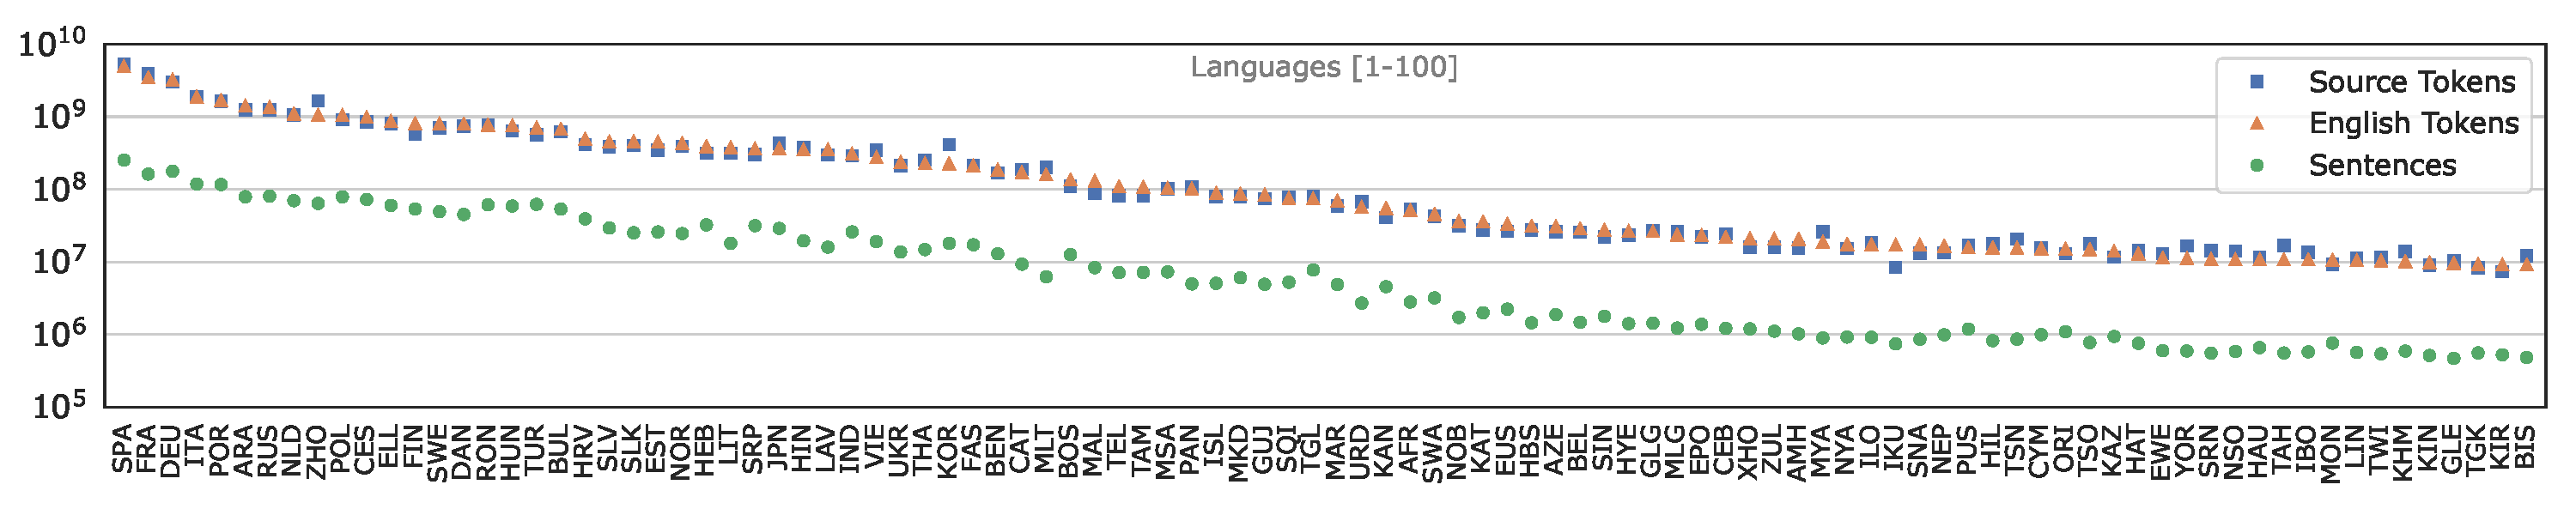
\includegraphics[width=\linewidth,trim={5mm 5mm 6mm 5mm},clip]{img/manyeng/v2-lang-stats-1-100.pdf}
    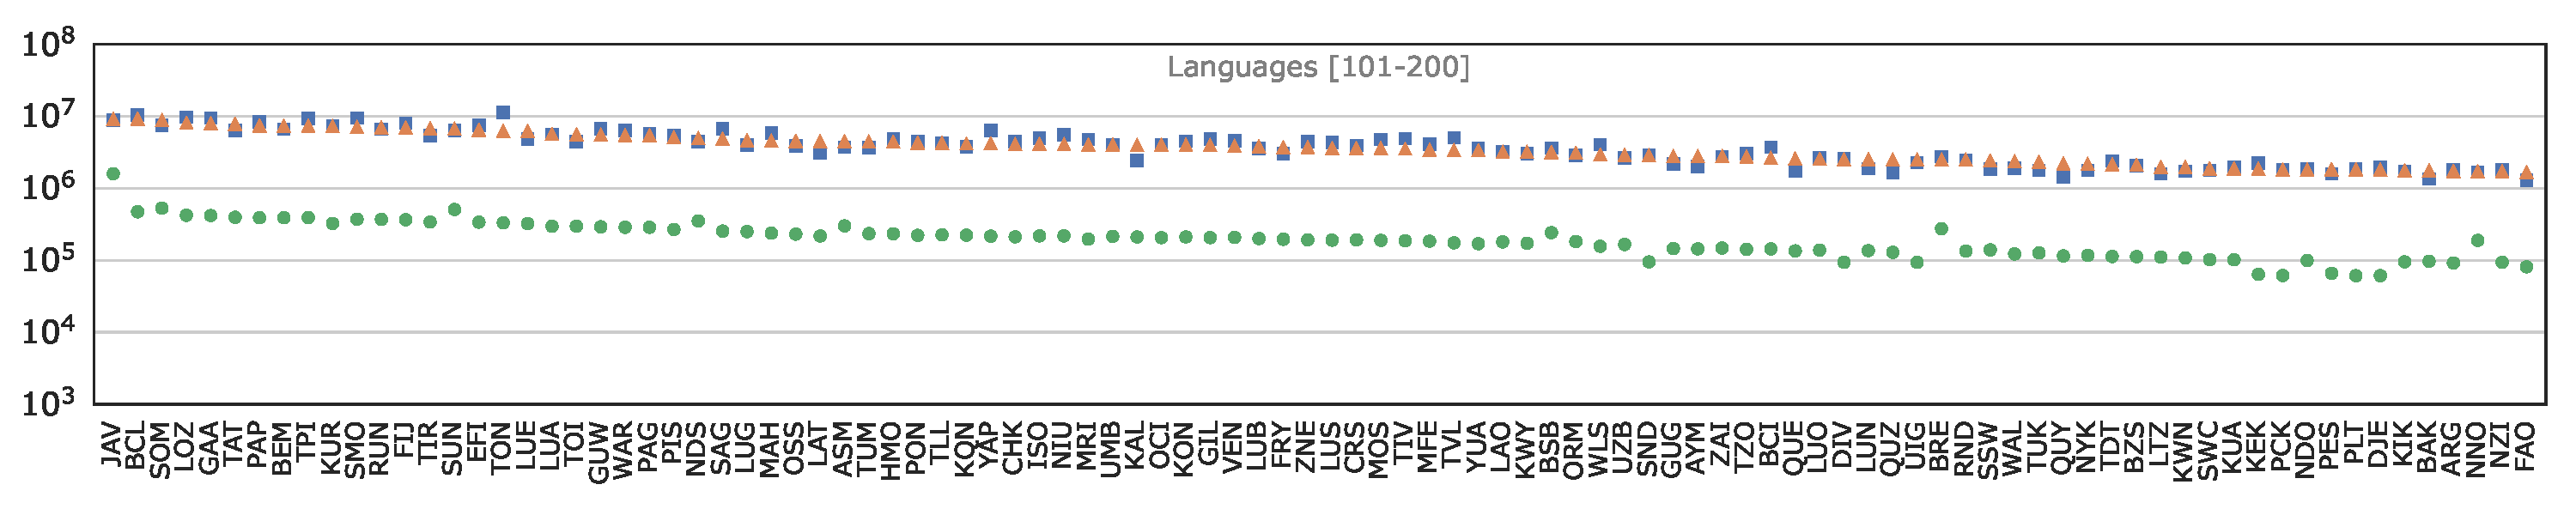
\includegraphics[width=\linewidth,trim={5mm 5mm 6mm 5mm},clip]{img/manyeng/v2-lang-stats-101-200.pdf}
    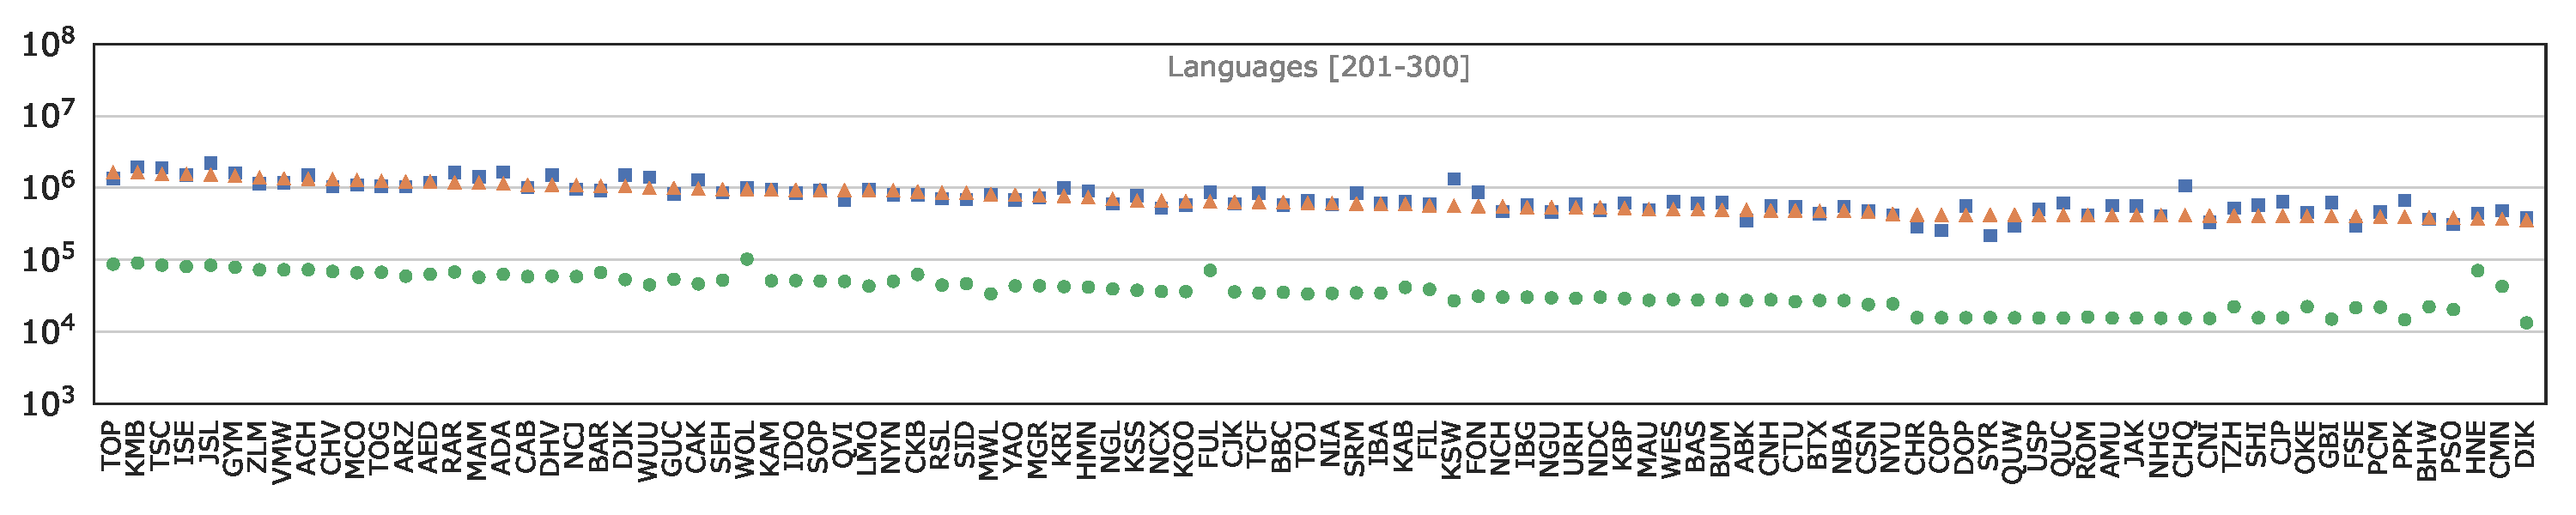
\includegraphics[width=\linewidth,trim={5mm 5mm 6mm 5mm},clip]{img/manyeng/v2-lang-stats-201-300.pdf}
    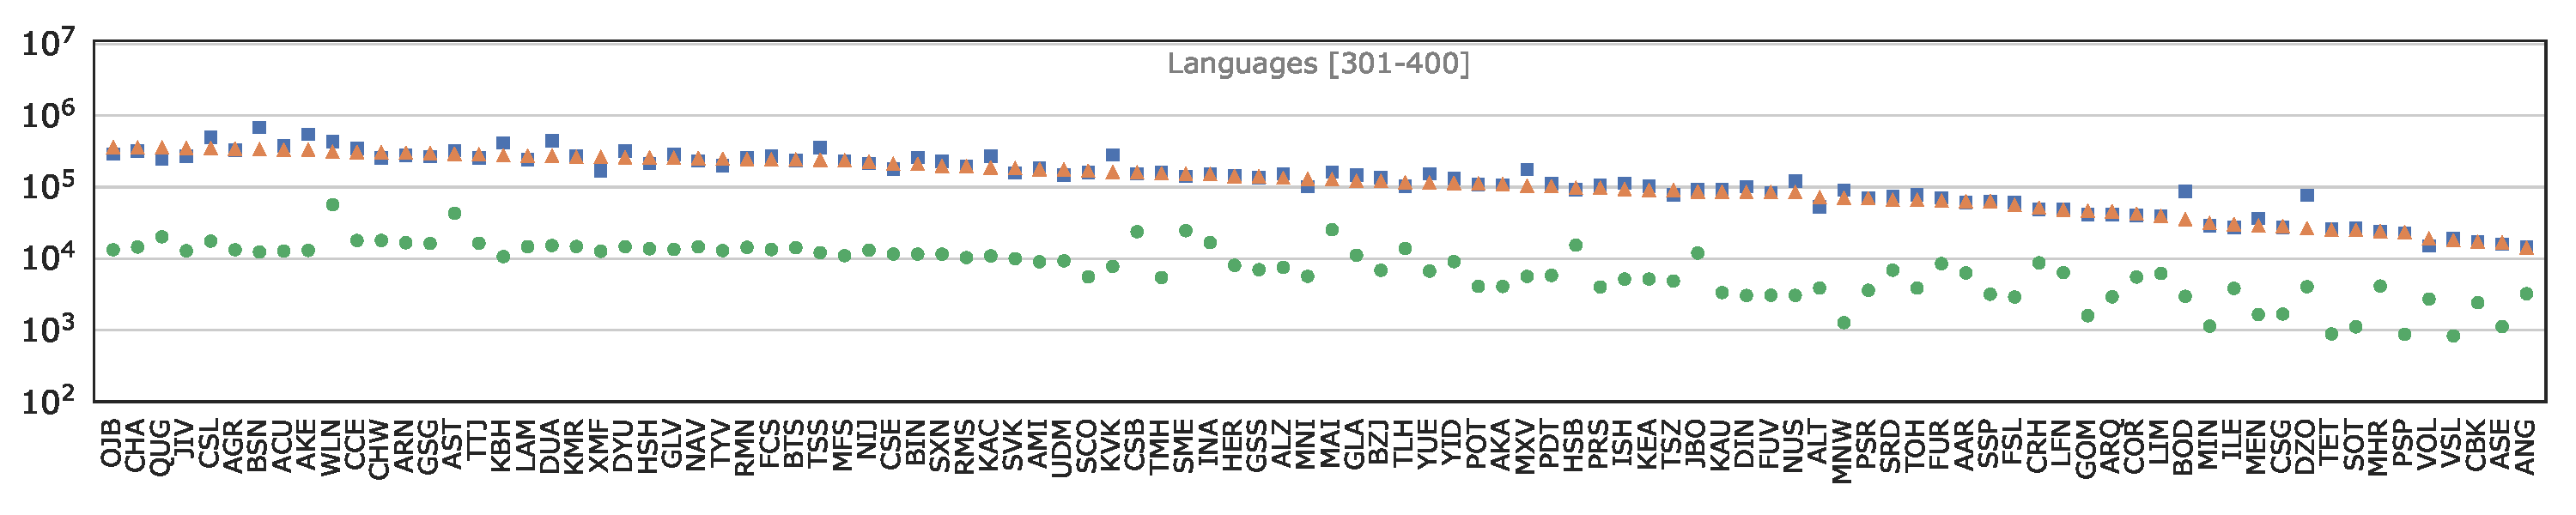
\includegraphics[width=\linewidth,trim={5mm 5mm 6mm 5mm},clip]{img/manyeng/v2-lang-stats-301-400.pdf}
    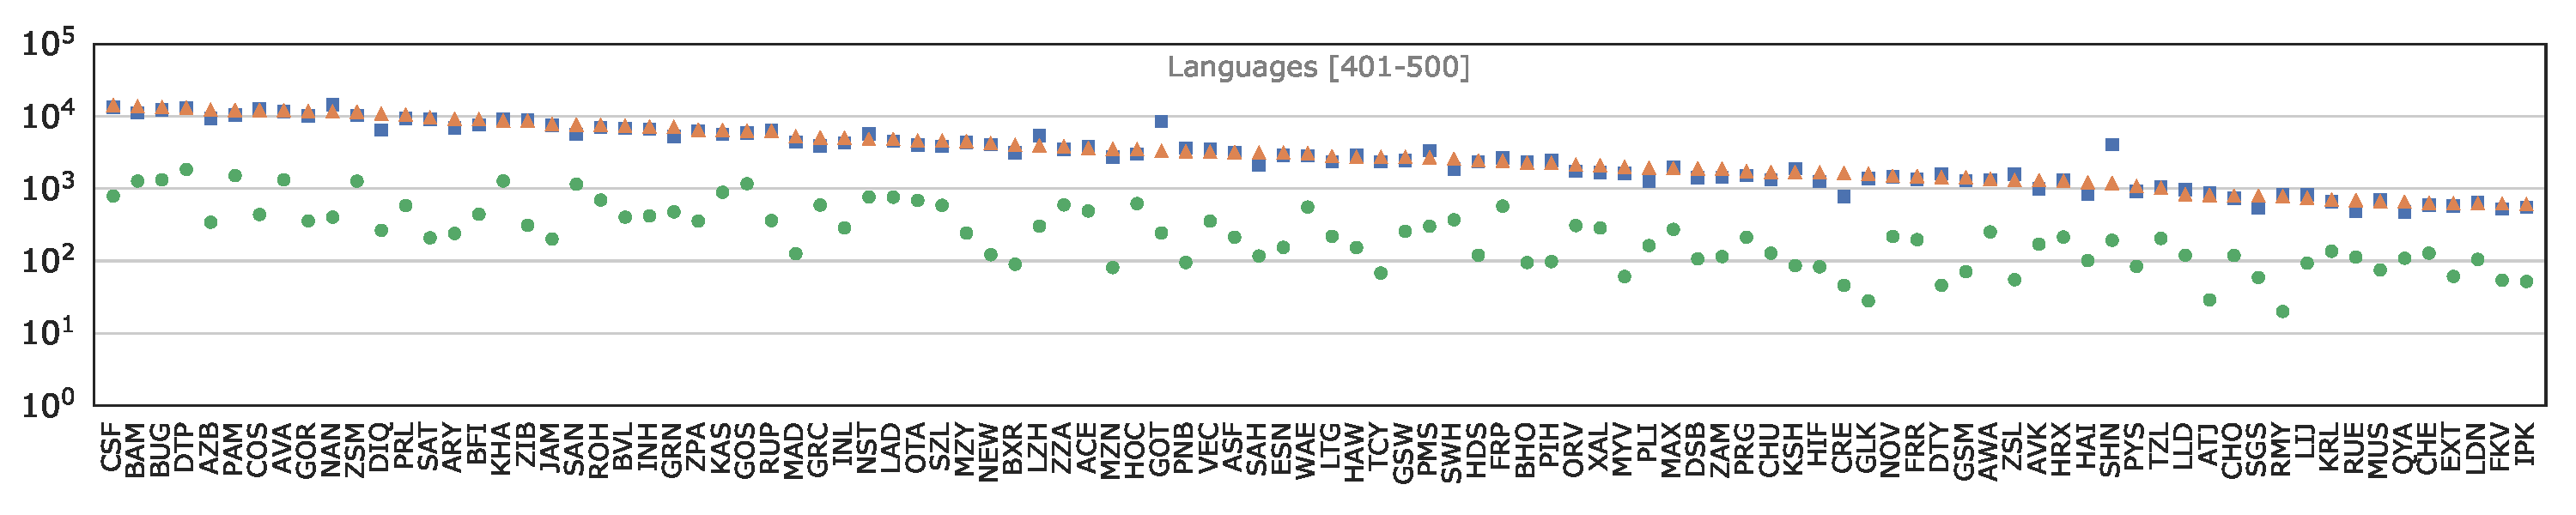
\includegraphics[width=\linewidth,trim={5mm 5mm 6mm 5mm},clip]{img/manyeng/v2-lang-stats-401-500.pdf}     
    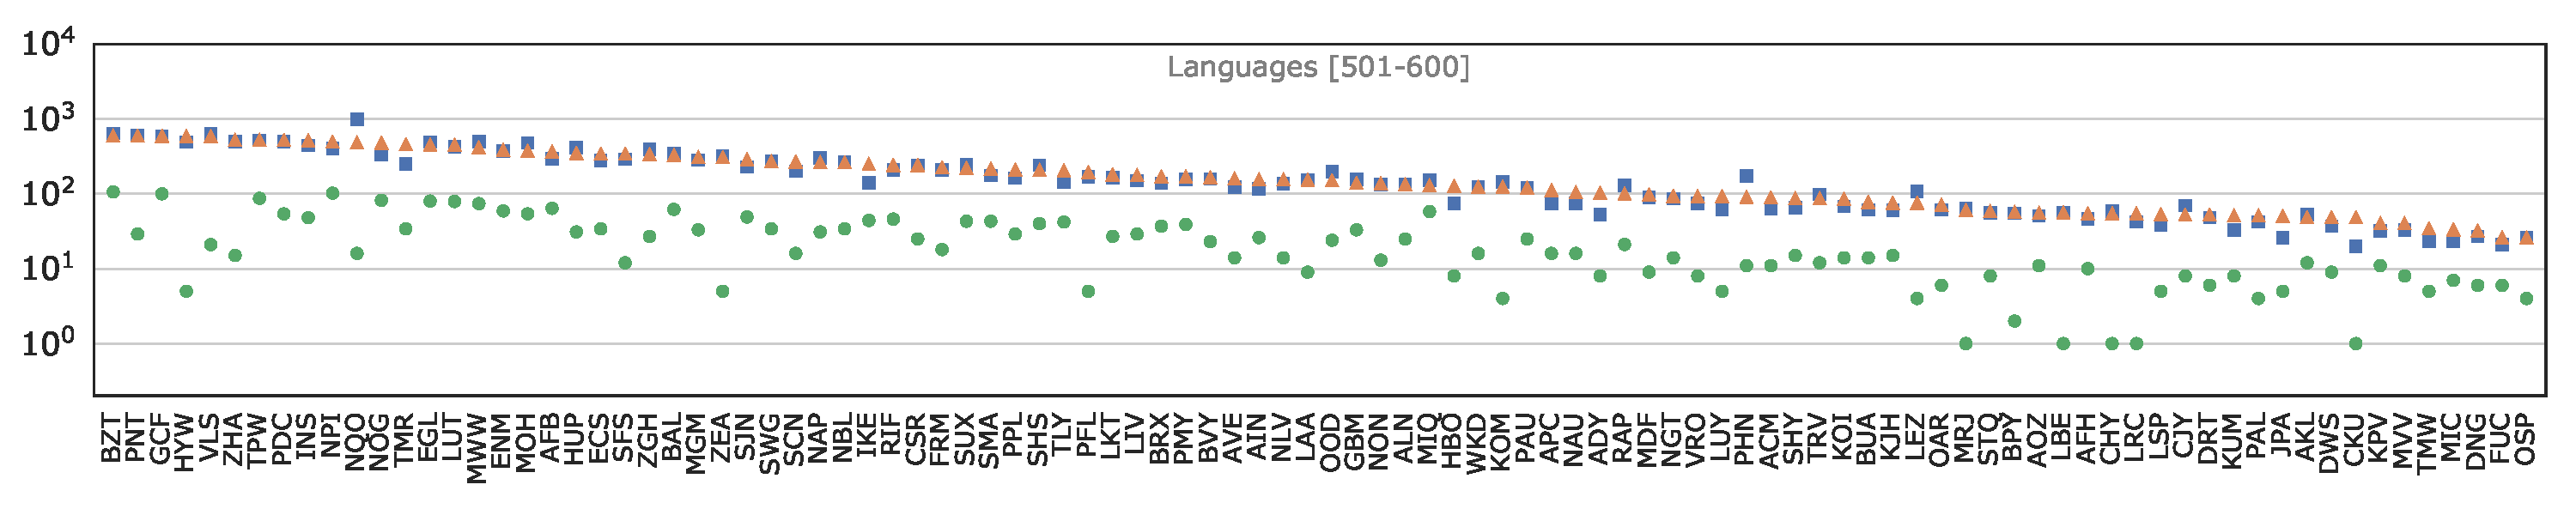
\includegraphics[width=\linewidth,trim={5mm 5mm 6mm 5mm},clip]{img/manyeng/v2-lang-stats-501-600.pdf}
    
    \caption{Training data statistics for 600 languages, sorted in descending order by English token count,  obtained after deduplication and filtering (see Section~\ref{sec:datasets}). The full name for these ISO 639-3 codes can be looked up using \mtdata, e.g. \texttt{mtdata-iso eng}.}
     \label{fig:train-data-stats-v2}
\end{figure*}

\subsection{Model}
Our V2 model has similar architecture as V1, which is a transformer with 9 encoders and 6 decoders, 512k source and 64k target vocabulary. Since the V2 training data is bigger than V1, our V2 model is made bigger: 1024 hidden dimensions, 4098 feed forward dimensions, and 16 attention heads. During training the V2 model, we use an effective mini batch size of 800k tokens, which is achieved using bfloat16 operations, gradient accumulations, and multiple GPUs. The training process achieved 74k optimizer updates in 3.5 days using 12 A100 GPUs (6 nodes x 2 each). The validation loss was still decreasing at that point. 

\subsection{Results}
As shown in Table~\ref{tab:many-eng-v2-scores}, the V2 model has consistent improvements across test sets: United Nations \cite{ziemski-etal-2016-unpc} which has 5 high resource languages, OPUS100 \cite{zhang-etal-2020-multiling-nmt} which cover 92 (medium-resource) languages, and WMT NewsTests \cite{bojar-etal-2017-findings,bojar-etal-2018-findings,barrault-etal-2019-findings,barrault-etal-2020-findings} having high quality test sets for 23  (mostly high resource languages). 

\begin{table}[ht]
\centering
\begin{tabular}{l l : rr:rr:rr} 
\hline 
\multicolumn{2}{r}{} & \multicolumn{2}{c:}{OPUS 100} & \multicolumn{2}{c:}{United Nations} & \multicolumn{2}{c}{WMT NewsTests} \\ \hline \hline 
\multicolumn{2}{l:}{Source Languages} & \multicolumn{2}{r:}{92} & \multicolumn{2}{r:}{5} & \multicolumn{2}{r}{23} \\
\multicolumn{2}{l:}{Segments; Src/Eng toks} & \multicolumn{2}{r:}{181.5k; 1.6M/1.7M} & \multicolumn{2}{r:}{20k; 474k/533k} 
      & \multicolumn{2}{r}{292.6k; 5M/6.1M} \\ \hline 
Version & Name & BLEU & MacroF1 & BLEU & MacroF1 & BLEU & MacroF1 \\ \hline \hline 
v1 & 500-Eng & 33.6 & 32.5 & 54.3 & 42.3 & 29.4 & 26.7 \\
v2 & 600-Eng & \textbf{34.2} & \textbf{33.2} & \textbf{55.7} & \textbf{44.1} & \textbf{32.4} & \textbf{32.5} \\
%v2.1 & v2 ft. on Code Switch & 32.4 & 32 & 54.3 & 42.5 & 30.7 & 31.2 \\ 
\hline 
\end{tabular} 
\caption{Multilingual NMT BLEU and MacroF1 scores. 
In addition to supporting more rare languages on the source side, the 600-English model has consistent improvements across on OPUS100 \cite{zhang-etal-2020-multiling-nmt} having test sets for 92 languages, United Nations \cite{ziemski-etal-2016-unpc} having 5 high resource languages, and WMT News Test \cite{barrault-etal-2020-findings} having high quality test sets for 23 languages. }
\label{tab:many-eng-v2-scores}
\end{table}

\subsection{Language Alternation Robustness}

In order to improve the multilingual NMT robustness for language alternations, we apply useful augmentation methods described in Section \ref{ch:rtobustness-sec:dataset}. 
Since the V2 dataset is already quite big, further augmentations at this scale results in prohibitively expensive cost. 
Hence, we select at most 200k random sentences per each language (i.e., down-sampling), which resulted in a corpus of 42.5M sentences in total. 
After augmenting with the two augmentation methods that proved effective in Chapter~\ref{ch:robustness} -- denoising, and random sentence concatenation -- on this smaller corpus, we obtained a parallel corpus of 130M segments. 
We fine-tuned the V2 model on this 130M sentence corpus (say V2.1 model), and evaluated on the same test sets as Section~\ref{ch:rtobustness-sec:dataset}. 
As shown in Table~\ref{tab:many-eng-v2-robustness}, the V2.1 model, although it takes a loss in Original test sentences, improves translation quality for inputs with partially translations (C-TL), missed sentence segmentations (C-SL), intersentential language alternations (C-XL), and random topic switching (R-XL). 

\begin{table}[ht]
    \centering
    \begin{tabular}{llrrrrr}
    \hline 
Version & Name & Orig & C-TL & C-SL & C-XL & R-XL \\ \hline \hline 
v1 & 500-Eng & 31.2 & 43.4 & 25.7 & 24.5 & 23.7 \\
v2 & 600-eng & \textbf{32.0} & 42.4 & 25.4 & 24.6 & 24.4 \\
v2.1 & v2+CodeSwitching & 29.6 & \textbf{62.9} & \textbf{30.5} & \textbf{29.9} & \textbf{29.8} \\ \hline 
\end{tabular} 
    \caption{Multilingual NMT's BLEU scores on language alternation datasets. These test sets are described in Section~\ref{sec:multiling-mt-checks} and statistics are given in Table~\ref{tab:heldout-stats}. 
    Data augmentation methods improve robustness to language alternation, however incur a little loss on the original single sentence translation quality.}
    \label{tab:many-eng-v2-robustness}
\end{table}


\section{Conclusion}

We have introduced our tools: \mtdata\ for downloading datasets, \nlcodec\ for processing, storing and retrieving large scale training data, and \rtg\ for training NMT models.
Using these tools, we have collected a massive dataset and trained a multilingual model for many-to-English translation.
We have demonstrated that our model can be used independently as a translation service, and also showed its use as a parent model for improving low resource language translation. 
We have also showed the effectiveness of data augmentation methods to improve the robustness of multilingual model to language alternations.  
All the described tools, used datasets, and trained models are made available to the public for free. 

%\section*{Acknowledgments}
%The authors would like to thank Lukas Ferrer, Luke Miles, and Mozhdeh Gheini for their contributions to some of the tools used in this work, and thank Jörg Tiedemann for hosting our prepared dataset at OPUS (\url{https://opus.nlpl.eu/MT560.php}). The authors acknowledge the Center for Advanced Research Computing (CARC) at the University of Southern California for providing computing resources that have contributed to the research results reported within this publication. URL: \url{https://carc.usc.edu}.  The authors acknowledge the Texas Advanced Computing Center (TACC) at The University of Texas at Austin for providing HPC resources that have contributed to the research results reported within this paper. URL: \url{http://www.tacc.utexas.edu}. This research is based upon work supported by the Office of the Director of National Intelligence (ODNI), Intelligence Advanced Research Projects Activity (IARPA), via AFRL Contract FA8650-17-C-9116.  The views and conclusions contained herein are those of the authors and should not be interpreted as necessarily representing the official policies or endorsements, either expressed or implied, of the ODNI, IARPA, or the U.S. Government. The U.S. Government is authorized to reproduce and distribute reprints for Governmental purposes notwithstanding any copyright annotation thereon.


\section*{Ethical Consideration}

\textit{Failure Modes:} \mtdata\ will fail to operate, unless patched, when hosting services change their URLs or formats over time.
On certain scenarios when a dataset has been previously accessed and retained in local cache, \mtdata\ continues to operate with a copy of previous version and ignores server side updates.
We have done our best effort in normalizing languages to ISO 639-3 standard and BCP-47b tags. 
Our multilingual NMT model is trained to translate a one or two \textit{full} sentences at a time without considering source language information; translation of short phrases without a proper context might result in a poor quality translation. 

\textit{Diversity and Fairness:}
We cover all languages on the source side for which any publicly available dataset exists, which happens to be about 500 source languages. 
Our model translates to English only, hence only English speakers benefit from this work. 


\textit{Climate Impact:}
\mtdata\ reduces network transfers to a minimum by maintaining a local cache to avoid repetitive downloads.
In addition to the raw datasets, preprocessed data is also available to avoid repetitive computation.
Our Multilingual NMT has higher energy cost than a typical single directional NMT model due to a larger number of parameters, however, since our single model translates hundreds of languages, the energy requirement is significantly lower than the total consumption of all independent models. 
Our trained models with are also made available for download.


\textit{Dataset Ownership:}
\mtdata\ is a client side library that does not have the ownership of datasets in its index.
Addition, removal, or modification in its index is to be submitted by creating an issue at \url{https://github.com/thammegowda/mtdata/issues}. 
We ask the dataset users to review the dataset license, and acknowledge its original creators by citing their work, whose \BibTeX\ entries may be accessed using:\\ \texttt{\footnotesize mtdata list -n <NAME> -l <L1-L2> --full} \\
The prepared dataset that we have made available for download includes \texttt{citations.bib} that acknowledges all the original creators of datasets.
We do not vouch for quality and fairness of all the datasets.
%JW300\cite{agic-vulic-2019-jw300} dataset was publicly available at the time of conducting the experiments, however, the authors have taken down the dataset at the time of writing this report.
